\documentclass[11pt]{article}
\usepackage[a4paper,margin=28mm]{geometry}
\usepackage[T1]{fontenc}
\usepackage{lmodern}
\usepackage{amsmath,amssymb,amsthm,mathtools}
\usepackage{microtype}
\usepackage{enumitem}
\usepackage{booktabs}
\usepackage[dvipsnames]{xcolor}
\usepackage{tikz}
\usetikzlibrary{arrows.meta,positioning}
\usepackage[colorlinks=true,linkcolor=MidnightBlue,citecolor=MidnightBlue,urlcolor=MidnightBlue,breaklinks=true]{hyperref}
\hypersetup{pdftitle={Milne's rationality conjecture for abelian varieties},
 pdfsubject={Rational pairings of specialized Hodge classes with Lefschetz classes},
 pdfauthor={OpenAI}}
\setlength{\emergencystretch}{2em}
\setlist[enumerate]{itemsep=3pt,topsep=5pt}
\setlist[itemize]{itemsep=3pt,topsep=5pt}
\newtheorem{theorem}{Theorem}[section]
\newtheorem{proposition}[theorem]{Proposition}
\newtheorem{lemma}[theorem]{Lemma}
\newtheorem{corollary}[theorem]{Corollary}
\theoremstyle{definition}
\newtheorem{definition}[theorem]{Definition}
\theoremstyle{remark}
\newtheorem{remark}[theorem]{Remark}
\numberwithin{equation}{section}
\newcommand{\Q}{\mathbb Q}
\newcommand{\Z}{\mathbb Z}
\newcommand{\R}{\mathbb R}
\newcommand{\C}{\mathbb C}
\newcommand{\F}{\mathbb F}
\newcommand{\Qbar}{\overline{\mathbb Q}}
\newcommand{\Kzero}{K_0}
\newcommand{\Cw}{C_w}
\DeclareMathOperator{\End}{End}
\DeclareMathOperator{\Hom}{Hom}
\DeclareMathOperator{\Tr}{Tr}
\DeclareMathOperator{\Fil}{Fil}
\DeclareMathOperator{\Res}{Res}
\DeclareMathOperator{\GSp}{GSp}
\DeclareMathOperator{\GL}{GL}
\DeclareMathOperator{\SL}{SL}
\DeclareMathOperator{\SU}{SU}
\DeclareMathOperator{\MT}{MT}
\DeclareMathOperator{\Lef}{Lef}
\DeclareMathOperator{\NS}{NS}
\DeclareMathOperator{\Gal}{Gal}
\DeclareMathOperator{\id}{id}
\DeclareMathOperator{\Spec}{Spec}
\title{Milne's rationality conjecture\protect\\ for abelian varieties}
\author{OpenAI}
\date{October 7, 2026}
\begin{document}
\maketitle
\vspace{-1em}
\begin{abstract}
We prove Milne's rationality conjecture for abelian varieties, including
residue characteristic \(2\). After good reduction, the pairing of a
rational Hodge class with any complementary product of divisor classes
on the reduction is the same rational number in every prime-to-\(p\)
realization and in crystalline cohomology. Using the Hodge theorem for CM
abelian varieties, we also show that every such specialized Hodge class
is represented by a single rational algebraic cycle in all these realizations.
\end{abstract}
\section{Introduction}

Suppose an abelian variety has good reduction at a prime. A rational
algebraic cycle on the variety specializes to a cycle on the reduction.
Its intersection with any complementary product of divisors has a rational
degree, and every cycle-class realization computes that same number.
Milne's rationality conjecture asks for this conclusion when the original
class is only known to be a rational Hodge class. We prove it for every
residue characteristic.

The distinction matters because good reduction can acquire divisors that
do not lift to the original variety. Deligne's absolute-Hodge theorem gives
compatible realizations of the Hodge class, but does not by itself identify
its pairing with these new divisors as the degree of a rational cycle.
The conjecture isolates this rationality question from the stronger problem
of representing the Hodge class by an algebraic cycle.

Fix \(\Qbar\subset\C\), a prime \(p\), and a \(p\)-adic place \(w\)
of \(\Qbar\). Write
\[
 \F=\overline{\mathbb F}_p,\qquad
 \Kzero=\operatorname{Frac}W(\F),\qquad
 \Cw=\widehat{\Qbar}_w.
\]
We regard \(\Kzero\) and an algebraic closure of it as subfields of
\(\Cw\). Good reduction means good reduction after descent to a number
field and finite extension at the chosen place.

\begin{theorem}\label{thm:main}
Let \(A/\Qbar\) be an abelian variety of dimension \(d\) with good
reduction \(A_0/\F\) at \(w\). Let \(0\leq r\leq d\), and let
\[
 \gamma\in H^{2r}(A(\C),\Q(r))
\]
be a rational Hodge class. For every list of Cartier divisors
\(D_1,\ldots,D_{d-r}\) on \(A_0\), there is a number \(q\in\Q\)
such that
\begin{align*}
 \Tr_\ell\bigl(\gamma_{0,\ell}
       c_{1,\ell}(D_1)\cdots c_{1,\ell}(D_{d-r})\bigr)&=q
       &&\text{in }\Q_\ell\quad(\ell\ne p),\\
 \Tr_p\bigl(\gamma_{0,p}
       c_{1,\mathrm{cris}}(D_1)\cdots
       c_{1,\mathrm{cris}}(D_{d-r})\bigr)&=q
       &&\text{in }\Cw.
\end{align*}
Here \(\gamma_{0,\ell}\) is the smooth proper specialization of the
\(\ell\)-adic realization, and \(\gamma_{0,p}\) is the
de Rham--crystalline specialization in
\[
 H^{2r}_{\mathrm{cris}}(A_0/W(\F))[1/p](r)
       \otimes_{\Kzero}\Cw.
\]
The traces use the top Tate twist and send the class of a zero-cycle to
its degree. If \(r=d\), the divisor product is \(1\).
\end{theorem}

By linearity the same conclusion holds for every rational Lefschetz class
of complementary codimension, that is, every rational linear combination
of products of divisors. The number \(q\) is common to all realizations
for the fixed data; no comparison between different reduction places is
required.

\subsection{Origins and consequences}

Milne introduced a weak-rationality formulation while studying the
reduction of Shimura varieties and the Langlands--Rapoport conjecture
\cite[Conjecture~6.1(A)]{Milne2000}. It asks that a specialized CM
Hodge class whose components lie in the local spans of divisor products
in every realization arise from one rational Lefschetz class.
The pairing formulation appears in his
AIM notes and his study of rational Tate classes
\cite[Section~10]{MilneAIM2007}, \cite[Conjecture~4.1]{Milne2009}.
A previous positive case is a CM abelian variety with simple ordinary
reduction, together with all its powers: in that case every divisor
class on the reduction lifts \cite[Example~4.2]{Milne2009}.

The broader purpose is to obtain rational cohomological correspondences
for abelian motives in characteristic~\(p\), compatible with reduction
from characteristic zero \cite[Sections~5--6]{Milne2000}; see also
\cite[Introduction and Section~2]{Milne2025}. For \(\ell\ne p\),
Tate classes are twisted \(\ell\)-adic classes fixed by a power of
Frobenius; there is a corresponding \(\Q_p\)-algebra of crystalline
Tate classes. A \emph{good theory of rational Tate classes} chooses
one graded \(\Q\)-algebra on each variety whose scalar extensions
give these Tate algebras. The theory is stable under pullback and
pushforward, contains divisor classes, and contains specializations of
CM Hodge classes \cite[Definitions~2.1 and~3.1]{Milne2009}.
These are cohomological correspondences; their definition does not
assert that they are algebraic.

Milne proved that the rationality assertion for all CM abelian varieties
is equivalent to the existence of such a good theory on varieties over
\(\F\) whose connected components are products of abelian varieties
and projective spaces \cite[Theorem~4.5]{Milne2009}.
Our proof also expresses each specialized Hodge class as the pullback,
along a rational homomorphism of special fibers, of a specialized Hodge
class from a CM abelian variety. This extends the theory's
specialization property beyond the CM case.
In Corollary~\ref{cor:all-hodge-specialization}, every rational
Hodge class on a good-reduction abelian variety specializes to a unique
class in one fixed good theory. Its crystalline component gives the
stated specialization after extension to \(\Cw\).

A distinct additional input gives algebraicity on the special fiber.
Combining the same transport with the Hodge theorem for CM abelian
varieties \cite[Theorem~1.1]{OpenAICMHodge2026},
Corollary~\ref{cor:algebraic-specialization} represents each specialized
Hodge class by one rational algebraic cycle in all the stated
realizations. Its pairing with any complementary algebraic cycle is
therefore a rational intersection number. This consequence uses the CM
Hodge theorem; the proof of Theorem~\ref{thm:main} is independent of it.

\subsection{The method and its antecedents}

Three foundational results make this question accessible. Deligne proved
that every Hodge class on an abelian variety is absolute Hodge
\cite[Main Theorem~2.11]{Deligne1982}. Blasius established its compatibility
with \(p\)-adic comparison \cite[Theorems~0.3 and~5.3]{Blasius1994};
Moonen presents the Blasius--Wintenberger comparison theorem, with
Ogus's simplification, in the perfect-residue-field form needed for
the local auxiliary lifts below \cite[Theorem~5.6.3]{Moonen1998}. Milne's theory of
Lefschetz classes supplies a common rational divisor algebra with perfect
complementary pairing, independent of the Weil cohomology
\cite[Section~5]{Milne1999}.

The determinant classes used in the proof belong to the theory of Weil
classes developed by Weil, Deligne and Andr\'e; see
\cite[Section~4 and Endnotes~M.10--M.12]{Deligne1982}.
Andr\'e's refinement of the CM reduction expresses Hodge classes by
pullbacks from varieties of split Weil type \cite{Andre1992}; a detailed
account is \cite[Theorem~1]{Milne2020}. We prove directly the balanced
form of that reduction needed here in Lemma~\ref{lem:cm-reduction}.
Balanced signatures assert equal Hodge multiplicities at conjugate
embeddings; split Weil type also requires the associated Hermitian
form to have a half-dimensional isotropic subspace.
Andr\'e's later theory of motivated cycles establishes a broader
unconditional motivic setting for abelian Hodge classes
\cite[Theorem~0.6.2]{Andre1996}, without identifying them with algebraic
cycles.

For an imaginary quadratic field, Markman has proved algebraicity of
Weil classes on abelian fourfolds of Weil type and on abelian sixfolds
of split Weil type \cite[Theorem~1.2]{Markman2026}. These are
characteristic-zero algebraicity results. The pairing argument here
applies in arbitrary dimension and begins only with the Hodge class
and its good reduction.

There is also a direct antecedent for the lifting strategy. Milne asked
whether a specialized CM Hodge class and a divisor could be lifted
together, up to isogeny, to a CM variety, and explained the resulting
rationality implication \cite[Question~10.6 and Proposition~10.7]{MilneAIM2007}.
His current account gives a conditional criterion through weak lifting
of Lefschetz classes on CM Weil triples and describes the reduction
from general Hodge classes through CM varieties to Weil classes
\cite[Introduction, Question~2.17, and Theorem~2.18]{Milne2025}.
Our proof follows this general route, using two auxiliary varieties
with different purposes. The
first is CM; the second realizes a prescribed admissible filtration
over a local field and need not be CM. The necessary realization
machinery comes from Grothendieck--Serre--Tate deformation theory,
Tate's extension theorem, and the integral-model and local-Shimura
results of Kisin--Zhou and Pappas--Rapoport
\cite{Grothendieck1970,Tate1967,KisinZhou2025,PappasRapoport2024}.
For the prescribed filtration, we choose a framed local Shimura
point over its admissible period and use integral uniformization;
the required uniformization condition is supplied by
\cite[Corollary~6.3]{GleasonLimXu2026}. We state the precise inputs
where they enter and prove the connecting arguments for the
prescribed flag.

The contribution along this route is to construct a filtration that
preserves the extra divisor and then obtain a rational divisor identity
on its lift. A separate normalization by rational intersection numbers
makes the tensor transports simultaneous in all realizations.
Kisin--Zhou's compatibility theorem concerns Weil--Deligne
representations across coefficient fields
\cite[Theorem~1.2]{KisinZhou2025}; the additional issue here is the
rational value of a Hodge--divisor intersection.

The key step is a dichotomy for balanced Weil classes: either all the
complementary Lefschetz pairings vanish, or the specialized class is
itself a rational polynomial in divisors, simultaneously in every
realization.

\subsection{Proof overview}

The proof has four stages. The order below describes the deduction;
Sections~\ref{sec:transport}--\ref{sec:weil} establish its reusable
constructions before Section~\ref{sec:reduction} assembles them.

\paragraph{1. Transport to a CM variety.}
Corollary~\ref{cor:cm-transport} constructs a CM
abelian variety \(C/\Qbar\), a quasi-isogeny
\(a_{\mathrm{CM}}:A_0^n\to C_0\), and a rational Hodge class
\(\kappa\) such that
\[
 \gamma_0=(a_{\mathrm{CM}}j)^*\kappa_0,
\]
where \(j\) includes the first factor. This is one rational algebraic homomorphism on the
special fibers and one equality in every realization. Kisin--Zhou's
special-point theorem supplies the CM lift
\cite[Theorem~2.2.7]{KisinZhou2025}. The local tensors initially determine
similitude scalars; a ratio of rational divisor intersections shows
that all those scalars are the same rational number. This normalization
is what transports the original rational class, rather than a separate
local multiple in each cohomology theory.

\paragraph{2. Reduce CM classes to balanced Weil classes.}
Lemma~\ref{lem:cm-reduction} constructs rational-idempotent factors of
actual powers of \(C\). Their homology has rank \(2s\) over a CM field
\(E\), with signatures \((s,s)\) at every embedding, and their
polarizations induce conjugation on \(E\). Their Weil classes are the
rational forms whose components, after splitting \(E\), are top
alternating forms on individual \(E\)-eigenspaces. Pullbacks of these
Hodge classes span the given CM Hodge class over \(\Q\). Good reduction
is retained. Having one rational value for each complementary
Lefschetz pairing is preserved by rational pullback
(Lemma~\ref{lem:pairing-functorial}). It therefore remains to prove
that assertion for balanced Weil classes.

\paragraph{3. Find a divisor and a compatible filtration.}
For a balanced Weil variety \(Z\), let \(\dagger\) denote Rosati on its
reduction and consider
\[
 \mathcal U=\{u\in\End^0(Z_0):u^\dagger=u,\quad
                         ue=\bar e u\text{ for all }e\in E\}.
\]
Proposition~\ref{prop:weil} proves a dichotomy. If \(\mathcal U\) has no
invertible element, every complementary Lefschetz pairing of a
specialized Weil class is zero. If it has an invertible element, the
specialized Weil class is itself a simultaneous rational Lefschetz
class: one rational polynomial in divisors gives its class in every
realization. For the second branch, such a \(u\) supplies a divisor
\(D^u\) whose alternating form is nondegenerate on each \(E\)-eigenspace.
Theorem~\ref{thm:filtration} constructs a weakly admissible balanced
filtration on the fixed crystalline module that preserves \(E\), \(u\),
and the polarization. Generic transversality has a classical role in
admissible-filtration constructions
\cite[Theorem~1 and Lemmas~1.1--1.2]{FontaineRapoport2005}.
Here bounded-degree avoidance makes all the constrained choices over
one finite extension, and a maximality argument reduces the
weak-admissibility test to subobjects stable under the endomorphisms.

\paragraph{4. Lift the divisor and extract a rational identity.}
The second case of Proposition~\ref{prop:transport} realizes this flag
on a local auxiliary abelian variety \(B\), with a marked quasi-isogeny
\(a_{\mathrm{fl}}:Z_0^m\to B_0\). The prescribed flag makes the
first-summand projector, its algebraic \(E\)-action, and the transported
divisor filtered. These specified algebraic maps lift to \(B\).
After choosing an abstract complex realization of \(B\), polynomial
coefficient extraction expresses the relevant rational Betti Weil class
as a rational linear combination of divisor products
(Lemma~\ref{lem:weil-divisor-span}). The same rational identity specializes
in every realization. Pullback returns it to \(Z_0\), completing the
case of an invertible element in the dichotomy and, through the first two stages, the
main theorem.

Figure~\ref{fig:two-transports} separates the two lifts and their
special-fiber markings. Section~\ref{sec:preliminaries} fixes comparisons,
traces, and rational pullback. Section~\ref{sec:transport} proves both
transport alternatives; Section~\ref{sec:filtration} constructs the
prescribed flag; Section~\ref{sec:weil} proves the balanced-Weil dichotomy;
and Section~\ref{sec:reduction} proves the CM reduction and finishes the
argument.

\begin{figure}[tbp]
\centering
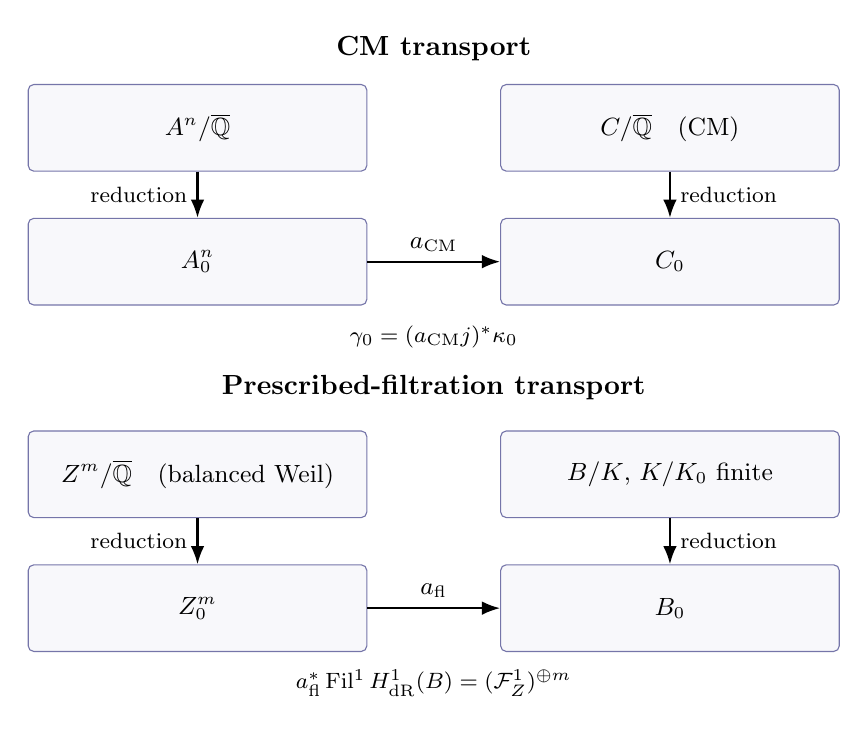
\begin{tikzpicture}[
 >=Latex, font=\small,
 variety/.style={draw=MidnightBlue!60,rounded corners=2pt,
                 fill=MidnightBlue!3,align=center,minimum width=43mm,
                 minimum height=11mm},
 every edge/.style={draw,->,thick},
 note/.style={font=\footnotesize,align=center}]
\node[font=\bfseries] at (3,1.0) {CM transport};
\node[variety] (A) at (0,0) {$A^n/\Qbar$};
\node[variety] (C) at (6,0) {$C/\Qbar$\quad(CM)};
\node[variety] (A0) at (0,-1.7) {$A_0^n$};
\node[variety] (C0) at (6,-1.7) {$C_0$};
\path (A) edge node[left,note] {reduction} (A0);
\path (C) edge node[right,note] {reduction} (C0);
\path (A0) edge node[above] {$a_{\mathrm{CM}}$} (C0);
\node[note] at (3,-2.65) {$\gamma_0=(a_{\mathrm{CM}}j)^*\kappa_0$};
\node[font=\bfseries] at (3,-3.3) {Prescribed-filtration transport};
\node[variety] (Z) at (0,-4.4) {$Z^m/\Qbar$\quad(balanced Weil)};
\node[variety] (B) at (6,-4.4) {$B/K$, $K/K_0$ finite};
\node[variety] (Z0) at (0,-6.1) {$Z_0^m$};
\node[variety] (B0) at (6,-6.1) {$B_0$};
\path (Z) edge node[left,note] {reduction} (Z0);
\path (B) edge node[right,note] {reduction} (B0);
\path (Z0) edge node[above] {$a_{\mathrm{fl}}$} (B0);
\node[note] at (3,-7.05)
 {$a_{\mathrm{fl}}^*\Fil^1H^1_{\mathrm{dR}}(B)
       =(\mathcal F_Z^1)^{\oplus m}$};
\end{tikzpicture}

\caption{The two uses of transport. Each lower horizontal arrow is one
actual quasi-isogeny preserving the specified tensors in all
realizations; the vertical arrows denote good reduction. There is no
claimed map between the generic fibers. The upper construction starts
from the original variety. The lower construction is applied separately
to a balanced Weil variety \(Z\) arising in the CM reduction; its lift
\(B\) realizes the chosen filtration \(\mathcal F_Z^{\oplus m}\) under
\(a_{\mathrm{fl}}^*\). The CM and prescribed-filtration auxiliaries need
not coincide.}
\label{fig:two-transports}
\end{figure}

\section{Comparisons and rational Lefschetz classes}
\label{sec:preliminaries}

We first put the realizations in Theorem~\ref{thm:main} in a common
notation and formulate its conclusion as a property of cohomology classes.
The essential functorial fact is that this property is preserved by rational
pullback. We also record the criterion that will lift an additional divisor
once a suitable Hodge filtration has been realized.

We work in the category of abelian varieties up to isogeny. Thus
\(\Hom^0(X,Y)=\Hom(X,Y)\otimes_\Z\Q\), and divisors may have rational
coefficients. Pullback by a rational homomorphism is defined on \(H^1\)
and extended to its exterior algebra. If \(Nf\) is an actual homomorphism,
then on \(H^{2r}\)
\begin{equation}\label{eq:rational-pullback}
 f^*=N^{-2r}(Nf)^*.
\end{equation}
This convention is the same in all realizations.

For an abelian variety \(X/\F\), set
\[
 k_\ell=\Q_\ell\quad(\ell\ne p),\qquad k_p=\Cw,
\]
and write \(H_v^{2r}(X)(r)\) for its \(\ell\)-adic cohomology if
\(v=\ell\ne p\), and for crystalline cohomology extended to \(\Cw\)
if \(v=p\). Cup products will usually be written without a cup symbol.
All trace maps and divisor classes have their cycle-class normalizations.
The Betti Tate line \(\Q(r)\) supplies the twists in the other
realizations through comparison. Thus \(\Tr_v\) is the trace on top
cohomology with its top Tate twist and sends the class of a zero-cycle to
its degree. For a good-reduction lift, \(\gamma_{0,\ell}\) denotes
smooth proper specialization of its absolute-Hodge realization, and
\(\gamma_{0,p}\) denotes de Rham--crystalline specialization extended
from \(\Kzero\) to \(\Cw\). We keep first crystalline cohomology
over \(\Kzero\) when constructing filtrations, and specify each
extension of the filtration field separately.

We use the exterior-algebra description of abelian cohomology and
faithfulness of rational homomorphisms on \(H^1\); see
\cite[Theorems~12.5 and~15.1]{MilneAV} for the prime-to-characteristic
realizations. The uniform Weil-cohomology formalism, including
crystalline cohomology, exterior powers, cycle-normalized traces and
the projection formula, is set out in
\cite[Section~1 and Appendix, Proposition~(A.2)]{Milne1999}. Smooth
proper specialization away from \(p\) is
\cite[Theorem~20.4]{MilneLEC}.

\subsection{Comparison of Hodge tensors}

\begin{lemma}\label{lem:comparison}
For an abelian variety with good reduction, the realizations of an
absolute Hodge class are compatible with the de Rham and crystalline
comparison isomorphisms. In particular, the \(p\)-adic crystalline tensor
obtained from its \(p\)-adic \'etale realization agrees, after extension of
scalars, with the de Rham--crystalline realization in
Theorem~\ref{thm:main}. These compatibilities respect tensor operations,
duals, Tate twists, divisor classes, and rational homomorphisms.

The same assertion applies to auxiliary abelian varieties with good
reduction over a finite extension of \(\Kzero\), using a complex
embedding of an algebraic closure of their field of definition.
\end{lemma}

\begin{proof}
For abelian varieties over \(\Qbar\), Deligne's absolute-Hodge theorem
\cite[Main Theorem~2.11]{Deligne1982} and Blasius's comparison theorem
\cite[Theorems~0.3 and~5.3]{Blasius1994} give the assertion. The
compatibility of the crystalline comparison with the de Rham comparison
is part of \cite[\S5.1]{Blasius1994}. The formulation for a complete
mixed-characteristic discrete valuation ring with perfect residue field
is given in \cite[Theorem~5.6.3]{Moonen1998}; the paragraph following
that theorem explains removal of the number-field hypothesis. A finite
extension of \(\Kzero\) is within that scope. The stated functorialities
are those of the comparison isomorphisms.
\end{proof}

An abstract complex embedding used here need not be continuous. To see
that it can be chosen compatibly with \(\Qbar\subset\C\), take a
transcendence basis of \(\overline{\Kzero}/\Qbar\), embed it in a
transcendence basis of \(\C/\Qbar\), and extend algebraically. The
cardinalities permit this construction. No descent of a general
auxiliary lift to \(\Qbar\) is inferred.

\subsection{The common rational Lefschetz space}

Let \(\Lef^r(X)\) be the space of rational polynomial expressions in
divisors of codimension \(r\), modulo numerical equivalence. We use the
following established properties:
\begin{enumerate}[label=(\roman*)]
 \item its cycle map is injective, and
 \(\Lef^r(X)\otimes_\Q k_v\) is the divisor-generated subspace of
 \(H_v^{2r}(X)(r)\);
 \item intersection and degree give a perfect pairing
 \[
   \Lef^r(X)\times\Lef^{\dim X-r}(X)\longrightarrow\Q;
 \]
 \item pushforward by a homomorphism of abelian varieties preserves the
 divisor-generated subspaces in each realization;
 \item hard Lefschetz and its inverse restrict to these subspaces.
\end{enumerate}
These are \cite[Proposition~5.2, Corollaries~5.3 and~5.5,
Theorem~5.9]{Milne1999}, with the author's correction to the proof of
Theorem~5.9. Crystalline cohomology is included. Extension of its
coefficient field to \(\Cw\) preserves these statements. We call the
tuple of realizations of a fixed element of \(\Lef^r(X)\) a
\emph{simultaneous rational Lefschetz class}.

\begin{definition}
A tuple \(\alpha=(\alpha_v)_v\), with
\(\alpha_v\in H_v^{2r}(X)(r)\), has the \emph{Lefschetz pairing
property} if, for every \(\delta\in\Lef^{\dim X-r}(X)\), the numbers
\(\Tr_v(\alpha_v\delta_v)\) are the images of one number in \(\Q\).
\end{definition}

Simultaneous rational algebraic classes have this property, by the
intersection formula. The property is closed under rational linear
combinations. We shall need the following additional closure property.

\begin{lemma}\label{lem:pairing-functorial}
If \(\alpha\) has the Lefschetz pairing property on \(Y\) and
\(f\in\Hom^0(X,Y)\), then \(f^*\alpha\) has that property on \(X\).
\end{lemma}

\begin{proof}
If \(r>\dim Y\), the input class is zero; if \(r>\dim X\),
its pullback is zero. We may therefore suppose that \(f\) is an actual
homomorphism and \(r\leq\min(\dim X,\dim Y)\).
For \(\delta\in\Lef^{\dim X-r}(X)\), the class \(f_*\delta_v\)
lies in the Lefschetz subspace of codimension \(\dim Y-r\) in every
realization. Choose rational bases \(a_i\) of
\(\Lef^{\dim Y-r}(Y)\) and \(b_j\) of \(\Lef^r(Y)\). The matrix
\(M_{ij}=\deg(a_i b_j)\) is an invertible rational matrix. If
\(f_*\delta_v=\sum_i c_{i,v}(a_i)_v\), the projection formula gives
\[
 \sum_i c_{i,v}M_{ij}=\deg(\delta f^*b_j).
\]
The right side is a rational number independent of \(v\). Solving this
one rational system shows that \(c_{i,v}=c_i\in\Q\) for every \(v\).
Thus \(f_*\delta\) is simultaneous rational Lefschetz. Applying the
projection formula once more proves the assertion. For rational \(f\),
use \eqref{eq:rational-pullback}.
\end{proof}

\subsection{Lifting a prescribed rational homomorphism}

The second transport construction will produce an abelian lift with a
chosen Hodge filtration. The following criterion then lifts the algebraic
projector, field action, and divisor already specified on its special fiber.
Its input is a rational algebraic homomorphism, rather than an arbitrary
map between cohomology spaces.

In the next lemma \(R\) is a complete mixed-characteristic discrete
valuation ring finite over \(W(\F)\), with fraction field \(K\).
For an abelian scheme \(\mathcal X/R\), the Hodge filtration is regarded
as a filtration of
\(H^1_{\mathrm{cris}}(X_0/W(\F))[1/p]\otimes_{\Kzero}K\).

\begin{lemma}\label{lem:lift-hom}
Let \(\mathcal X,\mathcal Y\) be abelian schemes over \(R\), with
special fibers \(X_0,Y_0\), and let
\(f_0\in\Hom^0(X_0,Y_0)\). If its contravariant crystalline map
preserves the Hodge filtrations, then \(f_0\) lifts uniquely to a
rational homomorphism \(\mathcal X\to\mathcal Y\).

In particular, a symmetric rational homomorphism \(X_0\to X_0^\vee\)
with this property lifts to a rational divisor class on the generic
fiber. Algebraic identities among finitely many such lifted maps remain
valid.
\end{lemma}

\begin{proof}
The crystalline map already commutes with Frobenius. Full faithfulness
for rational filtered Dieudonn\'e modules gives a rational morphism of
the associated \(p\)-divisible groups; see
\cite{Grothendieck1970} and the perfect-residue-field formulation in
\cite[\S4.2(v)]{IllusiePisa}. Equivalently, crystalline comparison first
gives the rational map on Tate modules. Multiply by an integer \(N\)
that clears both its Tate-lattice denominator and the denominator of
\(f_0\). Tate's extension theorem
\cite[Theorem~4]{Tate1967} extends the resulting integral generic-fiber
map of \(p\)-divisible groups over \(R\). Faithfulness of the
special-fiber Dieudonn\'e functor identifies its reduction with the
map induced by \(Nf_0\). Here equality after inverting \(p\) is
already equality of integral maps, because the integral Dieudonn\'e
modules are torsion free. The integer \(N\) is fixed for the remainder
of the construction.

The specified-map form of Serre--Tate deformation theory now gives a
lift over each \(R/\mathfrak m_R^n\)
\cite[p.~432]{Grothendieck1970}. One can also deduce it from the
fixed-object formulation \cite[Theorem~2.3.3]{IllusiePisa} as follows.
On \(X_0\times Y_0\) form the shear
\(s_0(x,y)=(x,y+Nf_0(x))\). The lifted \(p\)-divisible-group map gives
the same shear on the product \(p\)-divisible group. View the existing
product deformation with two special-fiber markings differing by
\(s_0\). Full faithfulness lifts the shear to an algebraic isomorphism
between these marked deformations; its second component restricted to
\(X\) lifts \(Nf_0\). Uniqueness makes these maps compatible at every
finite order.

Formal existence algebraizes the resulting formal map
\cite[Tag~0A42]{StacksProject}: its source is proper over the complete
noetherian ring \(R\), and its target is separated and of finite type.
Dividing by the fixed \(N\) gives the desired rational lift. Rigidity
gives uniqueness and injectivity of specialization on rational
homomorphisms \cite[Proposition~20.1 and Corollary~20.2]{MilneAV}.

If \(f_0\) is symmetric, injectivity shows that its lift is symmetric.
The usual identification
\[
 \NS(X_K)\otimes\Q
   \simeq\Hom(X_K,X_K^\vee)^{\mathrm{sym}}\otimes\Q
\]
gives the rational divisor class, after a finite extension if
necessary \cite[Proposition~17.2]{MilneAV}. Finally an identity between the maps specializes to the
given identity, so injectivity proves it upstairs as well.
\end{proof}

Only prescribed rational algebraic maps on the special fiber are being
lifted in Lemma~\ref{lem:lift-hom}. An arbitrary \(\Q_p\)-linear map of
\(p\)-divisible groups is not asserted to be a rational algebraic map.
We also use the extension of generic-fiber homomorphisms between abelian
schemes over a discrete valuation ring: their N\'eron mapping property
extends such a homomorphism uniquely over the base
\cite[Definition~5.1 and Example~5.3]{Conrad2003}. Clearing one
rational denominator therefore makes specialization of these maps
well defined.

\section{Transport through Hodge-type integral models}
\label{sec:transport}

After taking a power of the original abelian variety, we transport a
rational Hodge class to an auxiliary variety by one quasi-isogeny on
special fibers, with the same equality in every
realization. The auxiliary variety can be chosen either of CM type or
with a prescribed admissible Hodge filtration. These choices serve
different parts of the proof, but share the tensor construction and the
rational normalization in Proposition~\ref{prop:transport} below.

Throughout this section, a polarization on a rational homology space is
written as a rational alternating form, using the fixed Betti
trivialization of the Tate line.  If its similitude character is $c$,
an alternating form $\xi:V^{2r}\to\Q$ of multiplier $c^r$ means that
\begin{equation}
 \xi(gv_1,\ldots,gv_{2r})=c(g)^r\xi(v_1,\ldots,v_{2r}).
 \label{eq:transport-multiplier}
\end{equation}
Such a form is regarded as a tensor with its codimension-$r$ Tate
twist.  All homomorphisms and polarizations may be rational: an
isomorphism in the isogeny category induces the usual isomorphisms on
cohomology, including its tensor constructions.

We say that filtered isocrystal data have \emph{finite local-field
descent} if they are obtained by scalar extension from an isocrystal
with its tensors over the maximal unramified subfield \(H_0\) of a
finite extension \(H/\Q_p\), together with a filtration over \(H\).
The scalar extension is to \(\Kzero H\). This condition will let us
apply weak admissibility over a finite local field.
For a group in a faithful representation, a tensor-preserving
identification means one respecting a finite family of rational tensors
whose stabilizer is that group, together with their comparison realizations.

\begin{proposition}[Transport]
\label{prop:transport}
Let $A/\Qbar$ be an abelian variety of positive dimension with good
reduction at $w$, and put $V=H_1(A(\C),\Q)$. Suppose
\[
 G\subset\GSp(V,\psi)
\]
is connected reductive, its Hodge homomorphism $h$ gives the
Hodge structure of $A$, and its conjugacy class $X$ makes this
inclusion a Hodge embedding. Let $\gamma$ be a rational Hodge
class of codimension $r$, represented on $V$ by an alternating
form satisfying \eqref{eq:transport-multiplier}.

Then there exist a positive integer $n$, an auxiliary
good-reduction abelian variety $B$, a quasi-isogeny
$a:A_0^n\to B_0$, and a rational Hodge class $\kappa$ of
codimension $r$ on $B$ such that, for the first-factor inclusion
$j:A_0\to A_0^n$,
\begin{equation}
 (aj)^*\kappa_0=\gamma_0.
 \label{eq:transport-class}
\end{equation}
The equality holds simultaneously in every $\ell$-adic
realization with $\ell\ne p$ and in the crystalline realization
after extension to $\Cw$. Either of the following two further
specifications can be imposed.
\begin{enumerate}
\item The variety $B$ is of CM type and is defined over $\Qbar$,
with its indicated good reduction at $w$.
\item Put $D_A=H^1_{\mathrm{cris}}(A_0/W(\F))[1/p]$. Suppose
$\mathcal F_A$ is a filtration in degrees $0,1$ on $D_A$, over a
finite extension of $\Kzero$, which is weakly admissible and has
finite local-field descent together with the specialized tensors
specifying the $G$-structure. Suppose
also that, after a geometric tensor-preserving identification, it
lies in the $G$-orbit of the original Hodge filtration. Then $B$
can be defined over a finite extension $K/\Kzero$ inside $\Cw$,
and $a$ can be chosen so that
\begin{equation}
 a^*\Fil^1H^1_{\mathrm{dR}}(B/K)
       =(\mathcal F_A^1)^{\oplus n}.
 \label{eq:transport-prescribed-filtration}
\end{equation}
Here the equality is made after a common finite extension and
crystalline--de Rham identification. To discuss Hodge classes on
this $B$, choose a complex embedding of an algebraic closure of
$K$ extending the fixed embedding of $\Qbar$.
\end{enumerate}
In the second case the realizations of $\kappa$ are supplied by
the canonical tensor sections of the Hodge-type model and the
polarization. In the first case these agree with the usual
realizations and specialization of its absolute Hodge class.
\end{proposition}

We prepare two ingredients for the proof. First, we enlarge the given
Hodge datum so that integral-model theorems apply at every prime while
its rational representation remains a sum of copies of \(V\).
Second, we realize a prescribed admissible filtration by choosing a
framed local Shimura point above its crystalline period and applying
integral uniformization.  The resulting abelian lift retains that
point's integral tensors and special-fiber marking.  After these
preparations, the proof constructs the transported tensor and normalizes
it using rational divisor intersections.

\subsection{An auxiliary strongly admissible datum}

We recall the hypotheses on integral models that we will use.
For a reductive group \(H_p/\Q_p\), a full Bruhat--Tits stabilizer
is the smooth group scheme fixing a point of its extended building.
Its identity component is the associated parahoric group scheme.
Now let \((H,X_H)\) be a Shimura datum over \(\Q\). In the terminology
of \cite[Definition~2.1.6]{KisinZhou2025}, the triple
\((H,X_H,\mathcal H)\) is \emph{strongly admissible} if \((H,X_H)\)
is of Hodge type, \(\mathcal H\) is a full stabilizer of \(H_{\Q_p}\)
with connected special fiber, the centralizer of a maximal
\(\Kzero\)-split torus of \(H_{\Kzero}\) is \(R\)-smooth, and the
relative root system over \(\Kzero\) is reduced when \(p=2\).  Here $R$-smoothness is the condition on tori used in
\cite[\S2.4]{KisinZhouEarlier}.  We will use it only for products and
extensions of restrictions of scalars of split tori, for which it
holds by \cite[Proposition~2.4.6]{KisinZhouEarlier}.

\begin{lemma}[Auxiliary Hodge datum]
\label{lem:auxiliary-datum}
Let
\[
 (G,X)\lhook\joinrel\longrightarrow
 (\GSp(V,\psi),X_{\mathrm{Siegel}})
\]
be a Hodge embedding, with $G$ connected and similitude character $c$.
For every prime $p$ there exist a totally real field $P$, a connected
reductive group $J$, and a Hodge embedding
\[
 (J,X_J)\lhook\joinrel\longrightarrow
 (\GSp(W,\psi_W),X'_{\mathrm{Siegel}})
\]
with the following properties.
\begin{enumerate}
\item There are inclusions of Shimura data induced by
\[
 G\longrightarrow J\longrightarrow\Res_{P/\Q}G_P,
\]
where the first map is diagonal and $J$ is the subgroup on which the
similitude multipliers in the restriction of scalars agree.
\item The group $J_{\Q_p}$ is quasi-split and has a full connected
stabilizer $\mathcal J$ making $(J,X_J,\mathcal J)$ strongly admissible.
\item As a rational $J$-representation,
\begin{equation}
 W\simeq (V\otimes_{\Q}P)^{\oplus m}
 \label{eq:transport-copies}
\end{equation}
for some positive integer $m$.  The form $\psi_W$ has multiplier the
common character $c$, and $\mathcal J\to\GL(W_{\Q_p})$ extends to a
closed immersion into $\GL(\Lambda_p)$ for a self-dual $\Z_p$-lattice
$\Lambda_p$.
\end{enumerate}
\end{lemma}

\begin{proof}
Choose a finite extension of $\Q_p$ splitting $G_{\Q_p}$.  Polynomial
approximation, together with Krasner's lemma
\cite[Propositions~7.60--7.61 and Corollary~7.62]{MilneANT}, gives a
totally real number field $P$ whose completions at $p$ split $G_{\Q_p}$.  For
example, approximate the minimal polynomial of a primitive element
of a splitting extension at $p$, and a polynomial with distinct real
roots at the real place.  The resulting number field can have just
one place above $p$; this additional condition is not needed.

Define the multiplier fiber product
\begin{equation}
 J=(\Res_{P/\Q}G_P)
       \mathbin{\times}_{\Res_{P/\Q}\mathbf G_m}\mathbf G_m,
 \label{eq:equal-multiplier-group}
\end{equation}
where the last map is diagonal.  The Hodge cocharacter, or its
inverse according to convention, pairs to $1$ with $c$.  Since $c$
factors through $G^{\mathrm{ab}}$, its character on this torus is
primitive.  Thus $\ker(G^{\mathrm{ab}}\to\mathbf G_m)$ is a torus,
and $\ker(c:G\to\mathbf G_m)$ is connected reductive.  The exact
sequence
\[
 1\longrightarrow\Res_{P/\Q}(\ker c)_P
 \longrightarrow J\xrightarrow{c}\mathbf G_m\longrightarrow1
\]
proves connectedness and reductivity of $J$.  Moreover,
\begin{equation}
 J^{\mathrm{der}}=\Res_{P/\Q}G_P^{\mathrm{der}}.
 \label{eq:auxiliary-derived}
\end{equation}

The action on $U=V\otimes_\Q P$, with alternating form
$\Tr_{P/\Q}\psi_P$, gives a symplectic embedding of $J$ with
similitude character $c$.  The diagonal Hodge homomorphism gives
$X_J$.  The adjoint Hodge-type and Cartan-involution axioms follow
componentwise from those for $X$.  We also check that extending the
totally real field introduces no rational adjoint factor on which
the Hodge homomorphism is trivial.  Write a rational simple adjoint
factor as $\Res_{L/\Q}H$, with $L$ totally real.  Every field factor
$L'$ of $P\otimes_\Q L$ is totally real, and every real embedding of
$L$ extends to a real embedding of $L'$.  Hence the existence of a
nontrivial Hodge component for $H$ persists in each resulting
rational factor.  Finally the diagonal weight is rational and the
trace form is a polarization.  This proves that $(J,X_J)$ is a
Shimura datum of Hodge type.

Here are the local conditions explicitly.  Put $P\otimes\Q_p=
\prod_{v\mid p}P_v$ and choose a split maximal torus $T_v$ of
$G_{P_v}$.  The character $c$ on $T_v$ has a cocharacter section:
a conjugate of the Hodge cocharacter pairs to $1$ with it, and all
cocharacters of a split torus are defined over $P_v$.  The same
argument applies to $G_{P_v}^{\mathrm{ab}}$.  Consequently the
maximal torus of $J_{\Q_p}$ obtained from the $T_v$, and the
abelianization of $J_{\Q_p}$, have the forms
\begin{align}
 T_J&\simeq\mathbf G_m\times
       \prod_{v\mid p}\Res_{P_v/\Q_p}\mathbf G_m^{\operatorname{rk}G-1},
       \label{eq:auxiliary-torus}\\
 J_{\Q_p}^{\mathrm{ab}}&\simeq\mathbf G_m\times
       \prod_{v\mid p}\Res_{P_v/\Q_p}
                    \mathbf G_m^{\dim G^{\mathrm{ab}}-1}.
       \label{eq:auxiliary-abelianization}
\end{align}
The split Borels over the $P_v$ give a Borel of $J_{\Q_p}$, so this
group is quasi-split.  Its derived group is a product of restrictions
of split groups by \eqref{eq:auxiliary-derived}.  The vertices from
the hyperspecial vertices in those split groups give a very special
parahoric of $J_{\Q_p}$.  The inertia coinvariants of the cocharacter
module in \eqref{eq:auxiliary-abelianization} are torsion-free, since
that module is a direct sum of permutation modules.  The full
stabilizer is therefore connected by
\cite[Lemma~4.2.4]{KisinZhouEarlier}.

The centralizer of a maximal $\Kzero$-split torus is obtained from
\eqref{eq:auxiliary-torus} by unramified base extension; its torus
factors are still induced split tori and $\mathbf G_m$.
It is $R$-smooth by
\cite[Proposition~2.4.6]{KisinZhouEarlier}.  Finally restrictions of
split root systems give reduced relative root systems, also at
$p=2$.  These are precisely the strong-admissibility checks in the
construction of \cite[Proposition~5.3.8]{KisinZhou2025}.  They use
the stipulated Hodge embedding, not the assertion that $G$ is the
full Mumford--Tate group of a particular point.

Apply \cite[Proposition~2.1.9]{KisinZhou2025}, starting with the
representation $U$ just constructed.  Its proof first tensors $U$
with an auxiliary totally real $\Q$-vector space, then takes direct
sums, and finally applies the symplectic self-duality construction.
The group acts trivially on that extra vector-space factor.  In the
last construction the dual representation twisted by $c$ is
identified with $U$ by its symplectic form.  Thus every resulting
rational summand is a copy of $U$, with the same multiplier.  This
gives \eqref{eq:transport-copies}, together with $\psi_W$ and
$\Lambda_p$.  The assertion of the cited proposition includes
$p=2$; its proof uses the reduced-relative-root condition through
\cite[Lemma~2.1.8]{KisinZhou2025}.
\end{proof}

Choose a sufficiently small neat prime-to-$p$ level $K^p$ and put
$K_p=\mathcal J(\Z_p)$.  The adapted embedding gives the integral
model $\mathcal S_K$ and its universal abelian scheme.  A rational
$\Z_{(p)}$-lattice can be chosen with completion $\Lambda_p$.
We use a finite family of tensors defining its stabilizer
$\mathcal J$, as in \cite[\S2.1.4]{KisinZhou2025}.
Any additional rational $J$-invariant tensors may be included in
this family after clearing denominators.  Indeed their integral
stabilizer condition already holds on the generic fiber; flatness
of $\mathcal J$ makes it hold on $\mathcal J$ itself.  Adding them
therefore changes neither the group scheme nor its tensor
trivializations.

The added tensors have compatible sections in every realization, as
follows.  Use the homological degree-one realizations in this paragraph,
that is, the duals of the corresponding $H^1$, so that their reference
representation is $W$.  For such a realization $H_\nu$ over its
coefficient field $k_\nu$, let
\[
 \mathcal P_\nu=\operatorname{Isom}_{\{s_\alpha\}}
                    (W\otimes k_\nu,H_\nu)
\]
be its torsor of frames preserving the original defining tensors.
For a rational $J$-invariant tensor $u$ and a frame $e$, set
$u_\nu=e(u)$.  Two frames differ by an element of $J$, so this
definition is independent of the frame and descends from a
trivialization of the torsor.  It also works integrally after clearing
the fixed denominator of $u$.

The Betti and \'etale frame torsors are supplied by the canonical
tensor sections of \cite[\S2.1.4]{KisinZhou2025}.  The construction
of the universal Breuil--Kisin--Fargues module and its structure
tensors gives the crystalline torsor and its compatibility with
those sections
\cite[\S\S2.1.13--2.1.14]{KisinZhou2025}.
Indeed, a comparison map carrying every $s_\alpha$ to its specified
realization carries a frame $e$ to the comparison of $e$; it therefore
carries $e(u)$ to the same tensor evaluated in the new frame.
Thus it preserves $u_\nu$ for every added invariant $u$, without
requiring $u$ to be an expression in the chosen defining tensors.
At a lift over $\Qbar$, these are the realizations of its rational
Hodge tensor, by Lemma~\ref{lem:comparison}.  Their crystalline
specializations are independent of the lift because they are
evaluations in the fixed crystalline frame torsor.

The same observation applies to isogenies.  One quasi-isogeny
preserving the defining tensors identifies their frame torsors in
every realization in which those tensors are preserved.  It
therefore preserves all the added invariant tensors as well.
This proves the tensor comparison and simultaneous preservation
that will be used below; flatness alone is used only to keep the
integral stabilizer unchanged.

Specification~\textup{(1)} of Proposition~\ref{prop:transport}
uses the special-point theorem
\cite[Theorem~2.2.7]{KisinZhou2025} directly.  The next lemma is
needed only for specification~\textup{(2)}, where the filtration
has been prescribed in advance.

\subsection{Realizing a prescribed admissible filtration}

For a point $x\in\mathcal S_K(\F)$ let $C_x$ be the corresponding
abelian variety and put
\[
 \mathbb D_x=H^1_{\mathrm{cris}}(C_x/W(\F)),\qquad
 D_x=\mathbb D_x[1/p].
\]
The crystalline structure tensors are denoted $s_{\alpha,0,x}$;
the tensors away from $p$ are denoted $s_{\alpha,\ell,x}$.
They are the specializations of the canonical tensor sections and
are independent of the chosen lift of $x$.

The \emph{tensor isogeny class} $\mathcal I_x$ consists of the points
$y\in\mathcal S_K(\F)$ for which a single quasi-isogeny
$C_x\to C_y$ preserves $s_{\alpha,0}$ and every
$s_{\alpha,\ell}$ for $\ell\ne p$.  We emphasize that this
definition concerns actual quasi-isogenies of abelian varieties.
It is the class defined in \cite[\S2.2.4]{KisinZhou2025}.

\begin{lemma}[Realization of an admissible filtration]
\label{lem:admissible-realization}
Let $(J,X_J,\mathcal J)$ be strongly admissible, with $J_{\Q_p}$
quasi-split, and choose the adapted embedding and neat level above.
Let $x\in\mathcal S_K(\F)$ have a lift to characteristic zero.
Suppose a filtration $\mathcal F$ on $D_x$, after a finite extension
of $\Kzero$, has the following properties:
\begin{enumerate}
\item the resulting filtered isocrystal is admissible;
\item geometrically its filtration is induced by a $J$-valued
cocharacter in the conjugacy class prescribed by $X_J$.
\end{enumerate}
Then, after extending that field finitely, there are $y\in\mathcal I_x$,
a tensor-preserving quasi-isogeny $b:C_x\to C_y$, and a lift
$\widetilde y$ over the extended valuation ring such that
\[
 b^*\Fil^1 H^1_{\mathrm{dR}}(C_{\widetilde y})=\mathcal F^1
\]
under the crystalline--de Rham identification.

In particular, condition \textup{(1)} follows if the filtered
isocrystal and its tensor data have finite local-field descent and
$\mathcal F$ is weakly admissible.
\end{lemma}

\begin{proof}
Write $k=\F$ and let $\breve E$ be the completed local reflex field.
We work over a common finite extension $K$ of $\Kzero$ containing
$\breve E$ and a field of definition of $\mathcal F$.  Every further
field extension below is finite.  Put $K_p=\mathcal J(\Z_p)$.

We first fix the relation between the group and cohomological
conventions.  Let $\rho:J_{\Q_p}\to\GL(W_{\Q_p})$ be the adapted
homological representation and let $\rho^\vee$ be its dual.  Choose
the tensor-preserving identification
$\mathbb D_x\simeq\Lambda_p^\vee\otimes_{\Z_p}W(k)$ of
\cite[\S2.1.14]{KisinZhou2025}.  The local shtuka parameter is
$b_x\in J(\Kzero)$, whereas crystalline Frobenius on this
cohomological Dieudonn\'e module is
\[
 F_x=\rho^\vee(\sigma(b_x))\circ\sigma.
\]
The additional $\sigma$ on $b_x$ comes from the comparison with
the vector shtuka: its special-fiber module is
$(\sigma^{-1})^*(\mathbb D_x^\vee)$
\cite[Example~2.3.4 and Remark~2.3.10]{PappasRapoport2024}.
Write $\{\mu\}$ for the class prescribed by $X_J$; then
$[b_x]\in B(J,\mu^{-1})$.

For precision, identify the general linear crystalline period
flag with the appropriate filtration variety on $D_x$ by its
marked Rapoport--Zink interpretation.  If a deformation
$\mathcal H$ has special-fiber marking
$q:\mathcal H_k\dashrightarrow C_x[p^\infty]$, this identification
sends its period to
$(q^*)^{-1}\Fil^1H^1_{\mathrm{dR}}(\mathcal H)$.
Pushout through the faithful Hodge representation gives the
commutative period square
\[
\begin{array}{ccc}
M_{\mathcal J,b_x,\mu,K_p}&\longrightarrow&M_{\GL,\rho(b_x),\rho(\mu)}\\
\pi_{\mathrm{GM}}\downarrow&&\downarrow\pi_{\mathrm{GM}}\\
\mathcal F_{J,\mu}&\longrightarrow&\operatorname{Flag}(D_x).
\end{array}
\]
The lower map is a closed immersion: the parabolic stabilizing
the faithful filtration intersects $J$ in the parabolic for
$\mu$.  Define $f_{\mathcal F}$ to be the unique $J$-flag with
image $\mathcal F$.  It exists by condition~\textup{(2)}.  The
square uses crystalline periods and the dual Frobenius descent
above, so no extension of $\sigma$ to the ramified filtration
field is chosen.  When $q=b^{-1}$ its lower right period is
exactly $b^*\Fil^1$.

\medskip\noindent
\emph{A framed point over the prescribed period.}
Admissibility of the faithful filtered isocrystal implies that
the image of $f_{\mathcal F}$ in the general linear period flag
variety is in its admissible locus.  To see this in the
cohomological coordinates of the square, let $U$ be a crystalline
representation realizing $(D_x,\mathcal F)$.  Its crystalline
comparison identifies the associated vector bundle away from
the untilt with $U\otimes\mathcal O$.  The filtered de Rham
comparison identifies the modification at the untilt with the
standard lattice $U\otimes B_{\mathrm{dR}}^+$.  They glue to the
trivial bundle $U\otimes\mathcal O$ on the Fargues--Fontaine
curve, which is the general linear admissibility condition.
Since $\rho$ is faithful,
$\rho^{-1}(Z_{\GL(W)})\subset Z_J$: an element acting as a scalar
commutes with the faithful image of $J$.  The admissible-locus
identity in \cite[Proposition~3.1.1(i), (3.1.9)]{PappasRapoport2024}
therefore puts $f_{\mathcal F}$ in
$\mathcal F_{J,\mu}^{\mathrm{adm}}$.

This locus is the image of the crystalline period map
\[
 \pi_{\mathrm{GM}}:
 M_{\mathcal J,b_x,\mu,K_p}
       \longrightarrow\mathcal F_{J,\mu}^{\mathrm{adm}}.
\]
The map is \'{e}tale
\cite[\S3.1.1, (3.1.4)]{PappasRapoport2024}.
Its fiber at the classical point $f_{\mathcal F}$ is nonempty;
an \'{e}tale rigid space over $K$ has a point over a finite
extension of $K$.  After making that extension, choose
\begin{equation}
 z\in M_{\mathcal J,b_x,\mu,K_p}(K),
 \qquad \pi_{\mathrm{GM}}(z)=f_{\mathcal F}.
 \label{eq:transport-framed-point}
\end{equation}
In particular $z$ supplies the integral level as well as the
rational isocrystal marking.  If $C$ is the completed algebraic
closure of $K$, its moduli description gives an actual
$\mathcal J$-torsor $\mathcal P_z$, a Frobenius isomorphism
bounded by $\mu$, and, for sufficiently large $a$, an isomorphism
\[
 i_a:\mathcal J_{Y_{[a,\infty)}(C^\flat)}
      \xrightarrow{\ \sim\ }
      \mathcal P_z|_{Y_{[a,\infty)}(C^\flat)},
 \qquad
 \varphi_{\mathcal P_z}\circ\varphi^*i_a
       =i_a\circ\varphi_{b_x}.
\]
These are precisely the torsor and annular framing in
\cite[\S3.1.1]{PappasRapoport2024}.  Its associated
pro-\'{e}tale $\mathcal J(\Z_p)$-torsor gives integral tensor
frames.  Thus the integral structure and Frobenius-compatible
framing are part of the chosen point, with all their tensor
compatibilities.

\medskip\noindent
\emph{Integral realization and its special fiber.}
Our adapted datum is of global Hodge type: the group scheme is
a full connected Bruhat--Tits stabilizer, and the chosen Hodge
embedding is integral on $\Lambda_p$.
The center also satisfies the split-rank hypothesis of
\cite[\S4.1]{PappasRapoport2024}.  Indeed its real subgroup of
multiplier one preserves the positive definite form
$\psi_W(v,h(i)w)$ and is compact.  Its real split rank is
therefore at most one, while the rational weight torus supplies
one split central direction over $\Q$; both split ranks are one.
The model here is the one in
\cite[\S2.1.11 and Theorem~2.1.12]{KisinZhou2025}, obtained
from this adapted Hodge embedding and satisfying the
Pappas--Rapoport characterization.  Condition $(U_x)$ holds
by \cite[Corollary~6.3]{GleasonLimXu2026}; see also
\cite[Remark~4.10.4]{PappasRapoport2024}.  Consequently
\cite[Theorem~4.10.6]{PappasRapoport2024} represents the integral
local Shimura variety by a normal formal scheme
$\mathfrak M_{\mathcal J,b_x,\mu}$ and gives the morphism
\[
 \Theta_x:\mathfrak M_{\mathcal J,b_x,\mu}
          \longrightarrow\widehat{\mathcal S_K}.
\]
More precisely, \cite[\S4.10.2, (4.10.2)--(4.10.6)]{PappasRapoport2024}
identifies this formal scheme with the tensor-compatible open and
closed part of the pullback of the Siegel Rapoport--Zink space.
This construction identifies the pullback of the universal
$\mathcal J$-shtuka with its tautological framed shtuka and the
faithful vector realization with the universal $p$-divisible group.

Its rigid generic fiber is the local Shimura variety
\cite[Proposition~3.5.1(i)]{PappasRapoport2024}.
The classical point $z$ of this rigid generic fiber gives
$\operatorname{Spf}\mathcal O_K\to\mathfrak M_{\mathcal J,b_x,\mu}$.
Indeed it lies in the generic fiber of a formal affine chart;
for a special formal chart one may take an affinoid member of
its standard generic-fiber covering containing $z$.
Evaluation of the formal chart's ring is integral, and its
ideal of definition maps to topologically nilpotent elements of
$\mathcal O_K$.  Let $z_0$ be the special point and put
$y=\Theta_x(z_0)$ and $\widetilde y=\Theta_x(z)$.
The formal map $\widetilde y$ gives a point of the integral model
over $\mathcal O_K$ by restricting to an affine neighborhood of
$y$.  Pullback of the universal abelian scheme gives
$C_{\widetilde y}$ and its $p$-divisible group $\mathcal H_z$.

We record explicitly the integral comparison at this point.
For a uniformizer $\pi$ of $K$, put
$\mathfrak S=W(k)[[u]]$, with $u\mapsto\pi$, and let
$E_\pi(u)$ generate its kernel.  The crystalline representation
and integral level of $z$ give the $\mathcal J$-Breuil--Kisin
torsor of \cite[\S3.5]{PappasRapoport2024}, with
\[
 \Phi:\varphi^*\mathcal P_{\mathrm{BK}}[1/E_\pi]
             \xrightarrow{\ \sim\ }
             \mathcal P_{\mathrm{BK}}[1/E_\pi].
\]
Its pushout to $\GL(\Lambda_p)$ is the Breuil--Kisin module of
$\mathcal H_z$.  Reduction at $u=0$, followed by the dual
Frobenius descent fixed above, therefore gives the actual
Dieudonn\'e lattice of $\mathcal H_{z,k}$.
Proposition~3.5.1 of \cite{PappasRapoport2024} compares the two
specializations of this already constructed framed point.  In
the coordinates of \cite[Theorem~2.2.5]{KisinZhou2025} it gives
\[
 g\in X_{\mathcal J}(\mu^{-1},b_x),\qquad
 \mathbb D(\mathcal H_{z,k})
       =\rho^\vee(\sigma(g))\mathbb D_x\subset D_x.
\]
Indeed the Frobenius matrix on this lattice, written in its
induced basis, is
\[
 \rho^\vee\!\left(
       \sigma(g^{-1}b_x\sigma(g))\right)\circ\sigma,
\]
which explains the same Frobenius descent in the
Deligne--Lusztig condition and in the lattice formula.

\medskip\noindent
\emph{The abelian marking and the filtration.}
Keep the identity prime-to-$p$ coordinate in the uniformization.
The description of its special fiber in
\cite[\S4.10.3]{PappasRapoport2024}, or equivalently the
isogeny-class map of \cite[Theorem~2.2.5]{KisinZhou2025}, gives
$y=i_x(g)$ and a single abelian quasi-isogeny
$b:C_x\to C_y$ preserving the crystalline tensors and every
prime-to-$p$ tensor.  Its crystalline marking is the one just
used for $\mathcal H_z$, because the uniformization is induced
by the marked Siegel Rapoport--Zink space.

The crystalline period map of that space is the Hodge filtration
of its universal deformation pulled back by its marking.
Compatibility of $\Theta_x$ with the tautological shtuka and
\eqref{eq:transport-framed-point} consequently give
\[
 b^*\Fil^1H^1_{\mathrm{dR}}(C_{\widetilde y}/K)
       =\mathcal F^1.
\]
The deformation criterion
\cite[Proposition~2.2.3]{KisinZhou2025} is satisfied concretely:
the filtration is of type $\mu$, and the crystalline structure
tensors compare with the integral \'{e}tale tensors in the
$\mathcal J(\Z_p)$-frames of $z$.  The bounded integral shtuka
and its annular framing were obtained before using this
criterion or comparing specializations.  All cited global
Hodge-type and strongly admissible results apply at $p=2$ as
well.

Finally, under finite local-field descent, the weak-admissibility
inequalities restrict to the descended Frobenius subobjects.
Colmez--Fontaine's theorem
\cite[Theorem~A]{ColmezFontaine2000} makes those descended data
admissible, and scalar extension supplies condition~\textup{(1)}.
\end{proof}

\subsection{Proof of the transport proposition}

\begin{proof}[Proof of Proposition~\ref{prop:transport}]
\medskip\noindent
\emph{The original point and its reduction.}
Apply Lemma~\ref{lem:auxiliary-datum}.  Choose a rational
$J$-equivariant identification
$W=(V\otimes_\Q P)^{\oplus m}$ and set $n=m[P:\Q]$.
Choose a basis of $P$ whose first vector is $1$.  The resulting
identification of the Hodge structure at the diagonal point $h$
with $V^{\oplus n}$ makes the first-factor map equal to
\begin{equation}
 v\longmapsto(v\otimes1,0,\ldots,0).
 \label{eq:transport-first-factor}
\end{equation}
The rational homology/isogeny correspondence
\cite[Corollary~6.9]{MilneShimura} therefore makes the abelian variety
\(C\) at that point isogenous to \(A^n\). Fix a rational isogeny
\(f:A^n\to C\) realizing this identification.

We explain the field and reduction assertions for this starting
point.  The Hodge embedding maps it to the Siegel point of the
polarized variety $C$ with finite level.  The abelian variety $C$
is defined over $\Qbar$: clearing a denominator in $f$ realizes
it as a quotient of $A^n$ by a finite subgroup of its torsion, and
every such subgroup is defined over $\Qbar$.  Its rational
polarization and its finite level also descend to $\Qbar$, since
homomorphisms between abelian varieties over $\Qbar$ do not
enlarge after extending algebraically closed fields
\cite[Corollary~20.4]{MilneAV}.  The Hodge
embedding induces a finite morphism onto its
image at sufficiently small finite level
\cite[Theorem~5.16]{MilneShimura}. Its fiber over a
$\Qbar$-point therefore consists of $\Qbar$-points.  This places
the diagonal point on the canonical model over $\Qbar$.

After a finite number-field extension the variety $C$ has good
reduction, since it is isogenous to $A^n$
\cite[Chapter~IV, Theorem~3.5]{MilneAVNotes}.  Its polarization and
prime-to-$p$ level extend after a further finite extension.
The integral Hodge-type model is the normalization of the closure
of the generic fiber in the adapted Siegel model.  The valuative
criterion for this finite normalization therefore extends our
point to its integral model.  Denote the reduction by $x$.
The rational isogeny $f$ specializes to a quasi-isogeny
$f_0:A_0^n\to C_x$.

\medskip\noindent
\emph{The trace tensor and its descent.}
Next extend the alternating form defining $\gamma$
$P$-multilinearly and take its trace.  Composing with projection
onto the first copy in \eqref{eq:transport-copies} gives
\begin{equation}
 \eta=\Tr_{P/\Q}(\gamma_P)\circ
              (\operatorname{pr}_1)^{\otimes 2r}
       \in\bigwedge^{2r}W^*.
 \label{eq:transport-trace-tensor}
\end{equation}
For $r=0$ this is interpreted as the scalar trace.
The equal-multiplier condition implies that $\eta$ has multiplier
$c^r$ under $J$.  On \eqref{eq:transport-first-factor}, its
restriction is
\begin{equation}
 j^*f^*\eta_C=[P:\Q]\gamma.
 \label{eq:transport-trace-restriction}
\end{equation}
The class $\eta_C$ is understood with its Tate twist.

We turn this semi-invariant into the untwisted tensors to which
the integral-model theorems directly apply.  Write
$\psi_W^{-1}\in\bigwedge^2W$ for the inverse symplectic
bivector, and include
\begin{equation}
 u_\psi=\psi_W\otimes\psi_W^{-1},\qquad
 u_\eta=\eta\otimes(\psi_W^{-1})^{\otimes r}
 \label{eq:transport-untwisted-tensors}
\end{equation}
among the structure tensors.  Both are $J$-invariant tensors in
ordinary tensor constructions of $W$ and $W^*$; no separately
trivialized Tate object is needed.  They can be made integral and
added to the defining family as explained above.  Their
crystalline and prime-to-$p$ realizations at $x$ are the
specializations from the original point, with the comparison
conventions fixed above.

\phantomsection
\label{par:transport-tensor-descent}
The entire finite family of structure tensors, including
$u_\psi$ and $u_\eta$, has finite local-field descent.  To see
this, choose a finite extension $L/\Q_p$ over whose valuation
ring the original number-field point is defined, and let $L_0$
be its maximal unramified subfield.  The canonical \'etale
tensor sections of \cite[\S2.1.4]{KisinZhou2025}, pulled back
to that point, are $\Gal(\overline L/L)$-invariant.  Applying
the tensor functor $D_{\mathrm{cris},L}$ to these morphisms
from the unit object places them in the crystalline tensor
spaces over $L_0$.  Their extension to $\Kzero$ is exactly
the family $s_{\alpha,0,x}$, by good-reduction comparison.
The map $f_0$ also descends after a finite residue-field
extension, so this descent is retained under its marking.
Taking a compositum with the finite field of definition of a
prescribed filtration therefore gives one finite local field
for all the data.  No tensor-preserving trivialization over
$L_0$ is being asserted or needed.

\medskip\noindent
\emph{The two choices of lift.}
For specification~(1), apply
\cite[Theorem~2.2.7]{KisinZhou2025} to $x$.  It gives a point
$y\in\mathcal I_x$ with a special-point lift and a
tensor-preserving quasi-isogeny $b:C_x\to C_y$.
The special-point lift supplies a CM abelian variety $B$.  Special
points on the canonical Shimura variety are algebraic over its
reflex field by the canonical-model theory
\cite[Definition~12.8 and Proposition~14.14]{MilneShimura}, so $B$
and its level data can be taken over $\Qbar$.  The given local lift specifies their embedding at $w$
and their good reduction $B_0=C_y$.

For specification~(2), identify $D_x$ with $D_A^{\oplus n}$ using
$f_0^*$ and prescribe the direct-sum filtration
$\mathcal F_A^{\oplus n}$.  It is weakly admissible, with the
required finite local-field descent.  It is also in the required
$J$-cocharacter orbit.  Indeed a geometric element of the
transported $G$ taking the original filtration on $D_A$ to
$\mathcal F_A$ acts diagonally on all the copies of $V$ in $W$;
its image in $J$ takes the original filtration on $D_x$ to the
prescribed one.  The tensor-preserving identifications used here
come from the initial point and comparison, so they include the
$J$-structure tensors as well.  Geometric conjugacy can be
realized over a finite extension, since the corresponding
isomorphism scheme is of finite type.
Lemma~\ref{lem:admissible-realization} now gives $y$, its lift
$B$, and a tensor-preserving quasi-isogeny $b:C_x\to B_0$ with
the prescribed marked filtration.  This proves
\eqref{eq:transport-prescribed-filtration} for
$a=bf_0$.

\medskip\noindent
\emph{A common rational normalization.}
It remains, in both specifications, to recover the twisted class
and normalize it by a single rational scalar.  Choose a complex
description of the lifted Shimura point.  Its rational marking by
$W$ supplies a rational Hodge class $\eta_B$ corresponding to
$\eta$, and a rational divisor class $\theta_B$
corresponding to $\psi_W$.  Write $\theta_C$ for the analogous
class on $C$ and put
\[
 \theta_*=f_0^*\theta_{C,0}\in\NS(A_0^n)\otimes_\Z\Q.
\]
The class $\theta_*$ is rational ample.  Tensor preservation of
$u_\psi$ says that, in each realization,
\begin{equation}
 a^*\theta_{B,0}=\lambda_v\theta_*,
 \label{eq:transport-local-similitudes}
\end{equation}
with a nonzero local scalar $\lambda_v$.  Let $D=n\dim A$.
Pairing with $\theta_*^{D-1}$ gives
\begin{equation}
 \lambda_v=
 \frac{\deg\bigl(a^*\theta_{B,0}\cdot\theta_*^{D-1}\bigr)}
      {\deg(\theta_*^D)}=:\lambda\in\Q^\times.
 \label{eq:transport-rational-similitude}
\end{equation}
Both intersection numbers refer to rational divisor classes on
the same abelian variety; their cycle-class traces are identical
in every realization.  The denominator is positive because
$\theta_*$ is ample, and the numerator is nonzero by
\eqref{eq:transport-local-similitudes}.  Thus all the scalars in
\eqref{eq:transport-local-similitudes}, including the crystalline
one, are the single rational number $\lambda$.

Preservation of $u_\eta$, together with
\eqref{eq:transport-rational-similitude}, then yields
\begin{equation}
 a^*\eta_{B,0}=\lambda^r f_0^*\eta_{C,0}
 \label{eq:transport-eta-scaling}
\end{equation}
simultaneously.  In fact the inverse bivector scales by
$\lambda^{-1}$, so that the equality for the untwisted tensor
in \eqref{eq:transport-untwisted-tensors} gives exactly
\eqref{eq:transport-eta-scaling}.  Set
\[
 \kappa=\frac{\lambda^{-r}}{[P:\Q]}\eta_B.
\]
Specializing \eqref{eq:transport-trace-restriction} and using
\eqref{eq:transport-eta-scaling} proves
\eqref{eq:transport-class}.

For the arbitrary local lift, the crystalline realization just
used is unambiguous: the canonical model supplies the untwisted
tensor $u_\eta$, and the algebraic polarization supplies its Tate
line and inverse bivector.  The comparison isomorphism and these
operations define $\eta_B$ in the crystalline realization and
agree with its canonical \'{e}tale tensors.  Consequently any
identity expressing this class by algebraic divisor operations
specializes with the same rational coefficients in all
realizations.  For the $\Qbar$-valued CM lift, these are also the
usual absolute-Hodge and de Rham realizations.  This completes
the two constructions.
\end{proof}

\begin{corollary}[CM transport of a Hodge class]
\label{cor:cm-transport}
Let \(A/\Qbar\) be an abelian variety of positive dimension with
good reduction at \(w\), and let
\(\gamma\in H^{2r}(A(\C),\Q(r))\) be a rational Hodge class,
where \(0\leq r\leq\dim A\). There are a positive integer \(n\),
a CM abelian variety \(B/\Qbar\) with good reduction at \(w\),
a rational Hodge class \(\kappa\) of codimension \(r\) on \(B\),
and a quasi-isogeny \(a:A_0^n\to B_0\) such that
\[
 \gamma_0=(aj)^*\kappa_0,
\]
where \(j:A_0\to A_0^n\) is the first-factor inclusion. This is an
equality of the usual absolute-Hodge specializations in every
prime-to-\(p\) realization and in crystalline cohomology extended
to \(\Cw\).
\end{corollary}

\begin{proof}
Choose a polarization \(\psi\) on \(V=H_1(A(\C),\Q)\), and let
\(G=\MT(V)\). The Mumford--Tate group is connected reductive and
is characterized by its Hodge tensors
\cite[Section~3, Propositions~3.4 and~3.6]{Deligne1982}.
The Hodge homomorphism and its \(G(\R)\)-conjugacy class define
the Mumford--Tate Shimura datum of Hodge type, with faithful
symplectic representation
\[
 G\hookrightarrow\GSp(V,\psi).
\]
The polarization supplies the rational weight and the Cartan
involution condition. The definition of the Mumford--Tate group
excludes an adjoint factor on which the Hodge homomorphism is
trivial. The class \(\gamma\), with its Tate twist, is fixed by
\(G\). Equivalently, its alternating form on \(V\) has multiplier
\(c^r\), where \(c\) is the similitude character. Thus the first
alternative of Proposition~\ref{prop:transport} applies and gives
the asserted data and simultaneous equality.
\end{proof}

\section{An endomorphism-stable weakly admissible filtration}
\label{sec:filtration}

We construct a filtration on first crystalline cohomology that preserves an
additional divisor.  The construction takes place entirely on the given
isocrystal.  Its realization by an abelian lift will be a separate step.
Generic transversality is a basic ingredient of the admissible-filtration
existence theorems of Fontaine--Rapoport
\cite[Theorem~1 and Lemmas~1.1--1.2]{FontaineRapoport2005}.
We impose the additional endomorphism and polarization constraints
explicitly. The bounded-degree argument below chooses the required
coordinates over a finite algebraic extension, while testing every
subisocrystal over the fixed coefficient field.

Throughout this section, $\Kzero=\operatorname{Frac}W(\overline{\F}_p)$,
and valuations are normalized by $v(p)=1$.  If $D$ is an isocrystal over
$\Kzero$ and $K/\Kzero$ is finite, a subspace $L\subset D_K$ defines the
one-step filtration
\[
 \Fil^iD_K=
 \begin{cases}
 D_K,&i\leq 0,\\
 L,&i=1,\\
 0,&i\geq 2.
 \end{cases}
\]
For an isocrystal subobject $P\subset D$, its Hodge number for this
filtration is $t_H(P)=\dim_K(P_K\cap L)$.  Its Newton number $t_N(P)$ is
the sum of its slopes with multiplicities.  Weak admissibility means that
$t_H(D)=t_N(D)$ and $t_H(P)\leq t_N(P)$ for every isocrystal subobject
$P$ over $\Kzero$.

Finite local-field descent is understood as in Section~\ref{sec:transport}:
the isocrystal and its indicated tensors descend to the maximal unramified
subfield of a finite extension of \(\Q_p\), and the filtration descends
to that finite extension.

\begin{theorem}[The filtration construction]
\label{thm:filtration}
Let $A_0/\overline{\F}_p$ be an abelian variety equipped with a rational
action of a CM field $E$ and a polarization whose Rosati involution
restricts to conjugation on $E$.  Suppose that
\[
 D=H^1_{\mathrm{cris}}(A_0/W(\overline{\F}_p))[1/p]
\]
has rank $2s$ over $E\otimes_\Q\Kzero$, where $s\geq 1$.  Suppose also
that there is an invertible $u\in\End^0(A_0)$ such that
\[
 u^\dagger=u,\qquad ue=\bar e u\quad(e\in E).
\]
Let $\beta$ be the dual polarization pairing on $D$, with values in
the isocrystal line of slope $1$.

Then there are a finite extension $K/\Kzero$ and a subspace $L\subset
D_K$ with the following properties:
\begin{enumerate}
\item The one-step filtration with $\Fil^1D_K=L$ is weakly admissible.
\item $L$ is stable under the cohomological actions of $E$ and $u$,
and is Lagrangian for $\beta$.
\item After extending to an algebraically closed field $\Omega/K$,
one has $\dim_\Omega L_\tau=s$ for every embedding
$\tau:E\hookrightarrow\Omega$.
\item The isocrystal, its indicated tensors, and this filtration have
finite local field descent.
\end{enumerate}
Moreover, geometrically $L$ belongs to the balanced polarized
cocharacter orbit.  More explicitly, define
\[
 G_D=\left\{g\in\GSp(D,\beta)\cap
 \GL_{E\otimes_\Q\Kzero}(D):
 \det_{E\otimes_\Q\Kzero}(g)=c(g)^s\right\},
\]
where the scalar on the right is viewed in
$(E\otimes_\Q\Kzero)^\times$.  The balanced $E$-stable
$\beta$-Lagrangians form a single $G_D(\Omega)$-orbit.  Each is the
weight-$1$ space of a cocharacter of $G_{D,\Omega}$ with weights $0,1$.
In particular $L$ belongs to the orbit of any original filtration of
this type under a tensor-preserving comparison.
\end{theorem}

The proof will construct \(L\) from Lagrangians in finitely many
symplectic spaces. The two lemmas below supply the required simultaneous
choice: minimum intersection with a subspace is ensured by a nonzero
minor of bounded degree, and all such minors over a fixed coefficient
field can be made nonzero over one finite extension.

\begin{lemma}[Bounded-degree avoidance over a finite extension]
\label{lem:avoidance}
Let $K_1/\Kzero$ be a finite extension, and let $r,b\geq 1$ be integers.
There exist an element $\theta$ algebraic over $\Q_p$ and a point
\[
 (x_0,\ldots,x_{r-1})\in K_1(\theta)^r
\]
at which every nonzero polynomial in $K_1[X_0,\ldots,X_{r-1}]$ of total
degree at most $b$ is nonzero.  The coordinates $x_i$ can all be chosen
in $\Q_p(\theta)$.
\end{lemma}

\begin{proof}
Choose an integer $N>b$ and put
\[
 B=b\sum_{i=0}^{r-1}N^i.
\]
Let $e$ be the ramification index of $K_1/\Kzero$, so that
$v(K_1^\times)=\frac1e\Z$.  Choose a prime $q>\max(B,e)$, and choose
$\theta$ with $\theta^q=p$ in an algebraic closure of $K_1$.  The value
$v(\theta)=1/q$ has order $q$ modulo $\frac1e\Z$.  Consequently the
ramification index, and hence the degree, of $K_1(\theta)/K_1$ is at
least $q$.  The polynomial $X^q-p$ gives the reverse inequality, so
\[
 [K_1(\theta):K_1]=q>B.
\]

Set $x_i=\theta^{N^i}$.  Under the substitution $X_i=T^{N^i}$,
distinct monomials of total degree at most $b$ have distinct exponents:
each exponent of an individual variable is smaller than $N$, and
uniqueness follows from base-$N$ expansion.  Thus a nonzero polynomial
of total degree at most $b$ becomes a nonzero polynomial in $T$ of
degree at most $B$.  It cannot vanish at $\theta$, whose degree over
$K_1$ exceeds $B$.
\end{proof}

\begin{remark}
The coefficient field in Lemma~\ref{lem:avoidance} is the fixed field
$K_1$.  The conclusion concerns all bounded-degree polynomials over that
field, with no restriction on their cardinality.  It would be false with
$K_1(\theta)$ in place of $K_1$ as the coefficient field.
\end{remark}

\begin{lemma}[Intersections with Lagrangians]
\label{lem:lagrangian-intersection}
Let $M$ be a symplectic space of dimension $2m$ over a field $k$ of
characteristic zero, and let $W\subset M$ have dimension $a$.  A nonempty
open subset of the Lagrangian Grassmannian consists of subspaces $L$
such that
\[
 \dim(L\cap W)=\max(0,a-m).
\]
On any fixed symplectic affine big cell, at least one nonzero polynomial
of degree at most $m$ has nonvanishing locus contained in this open
subset.  This degree bound is independent of $W$.
\end{lemma}

\begin{proof}
We first work over an algebraic closure.  The Lagrangian Grassmannian
is geometrically integral of dimension $m(m+1)/2$; its affine big cells
are parametrized by symmetric $m\times m$ matrices.  If $1\leq a\leq m$,
consider the projective incidence variety of pairs $(\ell,L)$ with
$\ell\subset W$ a line and $\ell\subset L$ a Lagrangian.  The fiber over
$\ell$ is the Lagrangian Grassmannian of the symplectic space
$\ell^\perp/\ell$, and therefore the incidence variety has dimension
\[
 a-1+\frac{m(m-1)}2<\frac{m(m+1)}2.
\]
Its image is a proper closed subset.  Its complement consists precisely
of the Lagrangians missing $W$.  The case $a=0$ is immediate.  For
$a>m$, use
\[
 \dim(L\cap W)=a-m+\dim(L\cap W^\perp)
\]
and apply the preceding argument to $W^\perp$.

For the assertion on equations, choose coordinates on the fixed big
cell in which $L$ is the column space of
\[
 \begin{pmatrix}I_m\\ T\end{pmatrix},\qquad T=T^{\mathsf t}.
\]
The minimum-intersection condition says that the composite of this
matrix with the quotient map $M\longrightarrow M/W$ has rank
$\min(m,2m-a)$.  Its entries are affine linear polynomials in the
independent entries of $T$.  The nonempty open subset already proved
meets this big cell, so some minor of the required size is a nonzero
polynomial over $k$.  Its degree is at most $m$, and its nonvanishing
implies the required rank.  If the required rank is zero, use the
constant polynomial $1$.
\end{proof}


The two lemmas reduce simultaneous transversality to a uniform bound on
the degrees of the relevant minors. We now identify the symplectic
spaces on which to apply them and the inequalities they must enforce.

\begin{proof}[Proof of Theorem~\ref{thm:filtration}]
We write $e$ and $u$ also for their cohomological actions on $D$.
These actions commute with Frobenius and satisfy
\begin{equation}
\label{eq:filtration-adjoints}
 \beta(ux,y)=\beta(x,uy),\qquad
 \beta(ex,y)=\beta(x,\bar e y),\qquad ue=\bar e u.
\end{equation}
There is no change to the last relation from contravariance.  Indeed,
pulling back $ue=\bar e u$ gives $e^*u^*=u^*\bar e^*$; replacing $e$
by $\bar e$ gives $u^*e^*=\bar e^*u^*$.  Likewise, if $J$ is the
homological polarization matrix, $U^{\mathsf t}J=JU$ implies
$UJ^{-1}=J^{-1}U^{\mathsf t}$, which is the self-adjointness of the
cohomological action $U^{\mathsf t}$ for the dual pairing.  The
Rosati-conjugate adjoint identity for $E$ follows in the same way.

The pullback $U^{\mathsf t}$ of an individual endomorphism is
distinct from the contragredient group action $g\mapsto g^{-\mathsf t}$.
If a homological similitude $g$ has multiplier $c_V$ and satisfies
$\det_E(g)=c_V^s$, its dual action has multiplier $c_D=c_V^{-1}$
and satisfies $\det_E(g^{-\mathsf t})=c_D^s$.
Thus $G_D$ is the dual form of the homological group defined by this
determinant condition, with its cohomological multiplier.

\medskip\noindent
\emph{Reduction to the stable subobjects.}
First consider any $E,u$-stable candidate $L\subset D_K$, where
$K/\Kzero$ is finite. We show that the weak-admissibility inequalities
need only be tested on $E,u$-stable subobjects. This resembles the use of canonical
destabilizing objects in \cite[Section~2]{FontaineRapoport2005},
but we use total defect, not defect divided by dimension, and give
the required elementary argument.
For any isocrystal subobject $P\subset D$ over $\Kzero$, set
\[
 f(P)=t_H(P)-t_N(P).
\]
These values form a finite set: the Hodge number is a bounded integer,
and the Newton number is determined by bounded integer multiplicities
among the finitely many slopes of $D$.  Let $a$ be their maximum.
Newton numbers are additive in short exact sequences, while
\[
 (P_K\cap L)+(Q_K\cap L)\subset (P+Q)_K\cap L.
\]
Consequently
\begin{equation}
\label{eq:filtration-supermodularity}
 f(P)+f(Q)\leq f(P\cap Q)+f(P+Q).
\end{equation}
If $P$ and $Q$ both attain $a$, the right-hand terms are each at
most $a$, so both attain $a$.  Thus maximizers are closed under
intersection and sum.  Choose a maximizer $P_{\max}$ of largest
dimension.  Adding any other maximizer to it shows that the other
one is contained in it.  Hence $P_{\max}$ is the unique largest
maximizer.

The operators $u$ and $e\in E^\times$ are filtration-preserving
isocrystal automorphisms.  They preserve $f$ and hence fix
$P_{\max}$, by its uniqueness.  Thus $P_{\max}$ is $E,u$-stable.
Consequently, if $t_H(D')\leq t_N(D')$ for every $E,u$-stable
subobject $D'$, then $a=f(P_{\max})\leq0$. All the
weak-admissibility inequalities follow. We must therefore construct
an $E,u$-stable Lagrangian with these restricted inequalities and
$t_H(D)=t_N(D)$.

\medskip\noindent
\emph{Semisimplicity and symplectic blocks.}
The Rosati trace form
\[
 \langle a,b\rangle=\Tr(ab^\dagger)
 \quad\text{on }\End^0(A_0)\otimes_\Q\R
\]
is positive definite \cite[Theorem~17.3]{MilneAV}.  Left multiplication
by $u$ is self-adjoint for this form, since trace cyclicity gives
\[
 \langle ua,b\rangle=\Tr(uab^\dagger)
 =\Tr(ab^\dagger u)=\langle a,ub\rangle.
\]
It is therefore diagonalizable.  Its minimal polynomial equals the
minimal polynomial of $u$ in the endomorphism algebra, as is seen by
applying a polynomial in the multiplication operator to the identity.
Thus $u$, and hence $u^2$, acts semisimply on $D$.  The relation in
\eqref{eq:filtration-adjoints} also shows that $u^2$ commutes with $E$.

Put
\[
 B(x,y)=\beta(x,uy).
\]
This is a nondegenerate alternating pairing.  Indeed, invertibility is
immediate, and
$B(y,x)=-\beta(ux,y)=-B(x,y)$.  In addition,
\[
 B(ex,y)=\beta(x,\bar euy)=\beta(x,uey)=B(x,ey),
 \qquad B(u^2x,y)=B(x,u^2y).
\]
After a finite splitting extension $K_1/\Kzero$, write
\[
 D_{K_1}=\bigoplus_{\tau,z}M_{\tau,z},
 \qquad
 M_{\tau,z}=\{x:ex=\tau(e)x\ (e\in E),\ u^2x=zx\}.
\]
We omit zero summands.  The self-adjoint identities for $B$ show that
distinct summands are orthogonal.  Its restriction to each summand is
therefore nondegenerate.  Write $\dim M_{\tau,z}=2m_{\tau,z}$.

For $\bar\tau=\tau\circ\overline{(\cdot)}$, the operator $u$ maps
$M_{\tau,z}$ isomorphically to $M_{\bar\tau,z}$.  On these spaces,
\begin{equation}
\label{eq:filtration-u-similitude}
 B(ux,uy)=zB(x,y).
\end{equation}
Here $z\neq 0$, and $\tau\neq\bar\tau$.  Choose a $B$-Lagrangian
$L_{\tau,z}$ in one member of each opposite pair, and prescribe
\begin{equation}
\label{eq:filtration-opposite-choice}
 L_{\bar\tau,z}=uL_{\tau,z}.
\end{equation}
Equation~\eqref{eq:filtration-u-similitude} shows that the latter is
Lagrangian as well.  Their direct sum $L$ is $E$-stable and $u$-stable;
on applying $u$ twice, one obtains $zL_{\tau,z}=L_{\tau,z}$.  Since
\[
 \beta(x,y)=B(x,u^{-1}y),
\]
$L$ is also $\beta$-Lagrangian.  Its dimension at each $E$-embedding
is $s$.  It remains to make the independent choices appropriately.

\medskip\noindent
\emph{The inherited Newton grading.}
Use the canonical slope decomposition
\[
 D=\bigoplus_\lambda D_\lambda.
\]
The isocrystal category over $\overline{\F}_p$ is semisimple, and
this decomposition is functorial
\cite[\S3.2, Proposition~3.3]{ColmezFontaine2000}.  The slopes of $D$
belong to $[0,1]$: its integral Dieudonn\'e operators \(F,V\)
satisfy \(FV=p\), so both the slopes of \(F\) and those of \(V\)
are nonnegative.  All the endomorphisms above preserve every
$D_\lambda$, and the projectors onto the simultaneous eigenspaces
preserve its scalar extension.  Thus each block has a grading
\[
 M_{\tau,z}=\bigoplus_\lambda M_{\tau,z,\lambda},\qquad
 M_{\tau,z,\lambda}=M_{\tau,z}\cap(D_\lambda)_{K_1}.
\]
We use this grading even if Frobenius permutes the labels $(\tau,z)$.
No extension of Frobenius to $K_1$, and no isocrystal structure on an
individual block, is required.

Before scalar extension, $B$ is a pairing of isocrystals into the
slope-$1$ line.  Hence $B(D_\lambda,D_\mu)=0$ unless
$\lambda+\mu=1$.  Nondegeneracy on an individual block $M$ then gives
perfect pairings between $M_\lambda$ and $M_{1-\lambda}$.  In
particular, if $\dim M=2m$,
\begin{equation}
\label{eq:filtration-block-newton}
 \sum_\lambda\lambda\dim M_\lambda=m.
\end{equation}

Let $D'\subset D$ be an isocrystal subobject over $\Kzero$ stable
under $E$ and $u$.  Its intersections $M'=D'_{K_1}\cap M$ decompose
$D'_{K_1}$ and inherit the same slope grading.  Put $a=\dim M'$.
The slope sum of the graded quotient $M/M'$ is at most $2m-a$,
because all its slopes belong to $[0,1]$.  By
\eqref{eq:filtration-block-newton},
\begin{equation}
\label{eq:filtration-block-bound}
 \sum_\lambda\lambda\dim M'_\lambda
 \geq \max(0,a-m).
\end{equation}
The additional bound by zero follows from the nonnegative slopes.
The right side is also the smallest possible dimension of the
intersection of a Lagrangian in $M$ with $M'$.
Thus attaining this minimum in every block will give the
weak-admissibility inequalities for all the stable subobjects.

\medskip\noindent
\emph{Simultaneous choices and finite local field descent.}
We may arrange the splitting field and coordinates used above as
follows.  Choose a finite field $k_0\subset\overline{\F}_p$ over
which $A_0$, its polarization, $u$, and a rational basis of $E$ are
defined.  The underlying isocrystal and the indicated tensors then
descend to $\operatorname{Frac}W(k_0)$.  Choose a finite local field
$H/\Q_p$ containing this field and splitting the actions of $E$ and
$u^2$.  The eigenspaces and their symplectic bases can be constructed
over $H$ by linear algebra.  We take $K_1=\Kzero H$.  In particular,
the independent Lagrangian Grassmannians, fixed symplectic big cells
in them, and the maps induced by $u$ all have coordinates over $H$.

Take the product of these big cells, one for each independent choice
in \eqref{eq:filtration-opposite-choice}, and let $r$ be its number
of affine coordinates.  For every $E,u$-stable isocrystal subobject
$D'$ over $\Kzero$ and each independent block $M$, the space
$M'=D'_{K_1}\cap M$ is defined over the \emph{fixed} field $K_1$.
Lemma~\ref{lem:lagrangian-intersection} supplies a nonzero polynomial
over $K_1$, of degree at most $m$, whose nonvanishing ensures
\begin{equation}
\label{eq:filtration-minimal-intersection}
 \dim(L_{\tau,z}\cap M')=\max(0,\dim M'-m).
\end{equation}
We regard this as a polynomial on the whole product by ignoring the
other coordinates.  A single bound $b=\max m_{\tau,z}$ works for all
these polynomials, independently of $D'$.  On the opposite block,
the same intersection equality follows from $u$-stability of $D'$
and \eqref{eq:filtration-opposite-choice}.

Apply Lemma~\ref{lem:avoidance} to $K_1,r,b$.  Its one point satisfies
\eqref{eq:filtration-minimal-intersection} for every one of the
subobjects just specified, simultaneously.  This use of the lemma
does not assume that the collection of subobjects is countable or
that its members descend to $H$.  Their definition over $K_1$ and
the uniform polynomial degree bound are the only requirements.
There are nonzero blocks with $m\geq1$, so $r,b\geq1$ as required.

Put $K=K_1(\theta)=\Kzero H(\theta)$.  The resulting Lagrangian is
defined over $H(\theta)$ in the chosen coordinates, and $H(\theta)$
is finite over $\Q_p$.  Extending the original isocrystal to the
maximal unramified subfield of $H(\theta)$ therefore gives finite
local field descent of the complete filtered data.  In particular,
the construction has not obtained its generic point by introducing
transcendental parameters.

Summing \eqref{eq:filtration-minimal-intersection} and
\eqref{eq:filtration-block-bound} over all blocks gives
\begin{equation}
\label{eq:filtration-stable-test}
 t_H(D')\leq t_N(D')
 \quad\text{for every $E,u$-stable isocrystal subobject $D'\subset D$.}
\end{equation}
For $D$ itself, both numbers equal $\frac12\dim D$ by
\eqref{eq:filtration-block-newton}. The reduction to stable subobjects
proved at the start now gives all the weak-admissibility inequalities
for subobjects of $D$ over $\Kzero$. Each subobject over the smaller unramified
field of descent extends to one of these subobjects. Hence the
descended filtered isocrystal is weakly admissible as well.

\medskip\noindent
\emph{The geometric cocharacter orbit.}
Over $\Omega$, the polarization pairs $D_\tau$ only with
$D_{\bar\tau}$.  A balanced $E$-stable Lagrangian is determined by an
$s$-dimensional subspace of $D_\tau$ for one member of each pair;
the subspace in the opposite member is its annihilator.  The
subgroup of $G_D$ with multiplier $1$ contains the product of
$\SL(D_\tau)$ acting on opposite spaces by the inverse dual
representations.  These special linear groups are transitive on
the $s$-dimensional subspaces.  Thus all the indicated Lagrangians
form one $G_D(\Omega)$-orbit.

Finally choose an $E$-stable $\beta$-Lagrangian complement to one
such $L$.  Such a complement is obtained separately on each pair
of opposite embedding spaces.  Acting by $t$ on $L$ and by $1$
on the complement gives a cocharacter with multiplier $t$ and
$E$-determinant $t^s$ at each embedding.  It lies in $G_D$ and has
the stated filtration.  This proves the final assertions.
\end{proof}

\begin{corollary}
\label{cor:filtration-admissible}
The filtration of Theorem~\ref{thm:filtration}, with its finite local
field descent, is admissible: the descended filtered isocrystal is
the filtered crystalline module of a crystalline representation.
\end{corollary}

\begin{proof}
Apply the weakly-admissible-implies-admissible theorem of
Colmez--Fontaine with monodromy operator zero
\cite[Theorem~A]{ColmezFontaine2000}.
\end{proof}

\begin{corollary}[The divisor filtration condition]
\label{cor:filtration-divisor}
Let \(D,L\) be as in Theorem~\ref{thm:filtration}, and let \(\psi\)
and \(U\) denote the homological polarization and the homological
action of \(u\) on \(D_K^\vee\). The untwisted divisor form
\(\psi(\cdot,U\cdot)\) belongs to
\[
 \Fil^1\bigl(\bigwedge^2D_K\bigr)=L\wedge D_K,
\]
and hence to filtration degree zero after its codimension-one Tate
twist. If a marked power is realized by an abelian lift, the
corresponding pulled-back divisor satisfies the filtration condition
for its symmetric homomorphism in Lemma~\ref{lem:lift-hom}.
\end{corollary}

\begin{proof}
Let \(H\subset D_K^\vee\) be the annihilator of \(L\). It is
Lagrangian for \(\psi\) and stable under \(U\): for \(a\in L\)
and \(h\in H\),
\[
 a(Uh)=(u^*a)(h)=0.
\]
Therefore \(\psi(h,Uh')=0\) for \(h,h'\in H\). The divisor form
thus lies in
\[
 \ker\bigl(\bigwedge^2D_K\longrightarrow\bigwedge^2H^\vee\bigr)
       =L\wedge D_K.
\]
This proves the assertion on the fixed filtered vector space. After
realization of a marked power, pullback respects this filtration
condition, which is precisely the condition on the associated
symmetric homomorphism in Lemma~\ref{lem:lift-hom}.
\end{proof}

\section{Balanced Weil classes}\label{sec:weil}

Let $A/\Qbar$ have good reduction at the fixed place $w$, and let a CM
field $E$ act on $A$ up to isogeny.  We write $e\mapsto\bar e$ for its
complex conjugation.  Suppose that a polarization $\lambda$ induces this
involution on $E$.  Put
\[
 V=H_1(A(\C),\Q),\qquad \dim_E V=2s,\qquad
 g=\dim A=s[E:\Q],
\]
where $s\geq 1$.  We assume that the Hodge multiplicities at every
embedding of $E$ are $(s,s)$.  The polarization is an alternating form
$\psi:V\times V\longrightarrow\Q(1)$ satisfying
\[
 \psi(ex,y)=\psi(x,\bar e y).
\]

\begin{definition}\label{def:weil-space}
The rational space of \emph{Weil classes} associated with $E$ is the
subspace
\[
 W_E^s(A)\subset
 \bigwedge\nolimits_{\Q}^{2s} V^\vee\otimes\Q(s)
       =H^{2s}(A(\C),\Q(s))
\]
whose scalar extension to a splitting field $\Omega$ of $E$ is
\begin{equation}\label{eq:weil-pure-space}
 W_E^s(A)\otimes_\Q\Omega
 =\bigoplus_{\tau:E\hookrightarrow\Omega}
       \bigwedge\nolimits_\Omega^{2s}V_\tau^\vee
          \otimes\Q(s)_\Omega.
\end{equation}
Here each summand is extended by zero on the other eigenspaces.  The
right side is Galois stable, so it defines the indicated rational
subspace.
\end{definition}

The balanced multiplicities imply that every element of $W_E^s(A)$ is
a Hodge class: each determinant in \eqref{eq:weil-pure-space} has
untwisted type $(s,s)$.  We use its compatible realizations as an
absolute Hodge class; see \cite{Deligne1982}.  The same eigenspace
description of its support holds after specialization, since the
$E$-action specializes compatibly.

Our goal is the Lefschetz pairing property for these specialized
classes.  In fact, the reduction satisfies a dichotomy determined by
its rational endomorphisms.  Let $\dagger$ be Rosati for the reduced
polarization and put
\begin{equation}\label{eq:weil-U}
 \mathcal U=
 \{u\in\End^0(A_0):u^\dagger=u,\quad
                      ue=\bar e u\ \text{for every }e\in E\}.
\end{equation}

\begin{proposition}\label{prop:weil}
Every $\gamma\in W_E^s(A)$ satisfies the Lefschetz pairing property
at $w$.  More precisely, if $\mathcal U$ in \eqref{eq:weil-U} has no
invertible element, all complementary pairings are zero.  If it has
an invertible element, $\gamma_0$ is a simultaneous rational
Lefschetz class.
\end{proposition}

We first prove the vanishing alternative.  For the other alternative,
an invertible $u$ supplies a divisor whose form is nondegenerate on
each $E$-eigenspace separately.  We will lift this divisor and use it
to obtain a rational identity for the determinant classes.

\subsection{The orthogonality alternative}

\begin{lemma}\label{lem:weil-orthogonality}
If $\mathcal U$ contains no invertible element, every specialization of
a class in $W_E^s(A)$ is orthogonal to all complementary Lefschetz
classes, in each cohomological realization.
\end{lemma}

\begin{proof}
We prove the contrapositive.  A nonzero pairing will produce a divisor
form nondegenerate on one $E$-eigenspace.  We will then show that a
rational endomorphism in $\mathcal U$ with this property is invertible.

Fix one realization and extend its coefficient field to an
algebraically closed field $\Omega$.  At the crystalline component we
also include the coefficient extension used for the specialized
class.  In this proof, $V_\tau$ also denotes the corresponding
eigenspace in the dual of first cohomology of $A_0$, identified by
specialization and comparison.  Write $L^j_\Omega(A_0)$ for the $\Omega$-span of products of
$j$ divisor classes.  Since $[E:\Q]\geq2$, we have $g-2s\geq0$.
Hard Lefschetz on the Lefschetz algebra gives
\begin{equation}\label{eq:weil-hard-lefschetz}
 L^{g-s}_\Omega(A_0)
        =\psi_0^{g-2s}L^s_\Omega(A_0).
\end{equation}
The restriction of hard Lefschetz to this algebra, including for
crystalline cohomology, follows from the Lefschetz correspondences
of \cite[Theorem~5.9]{Milne1999}.

Suppose a Weil class pairs nontrivially with
$D_1\cdots D_s\psi_0^{g-2s}$, and choose a pure term, supported on
$V_\tau$, whose contribution is nonzero.  This term already has
degree $2s$ on $V_\tau$, so no further factor in a nonzero top-degree
product can use that space.  A factor from $\psi_0$ which uses
$V_{\bar\tau}$ also uses $V_\tau$; hence the polarization factors
contribute to neither space in this pair.  All $2s$ degrees on
$V_{\bar\tau}$ must therefore come from the $s$ divisor factors.
Each has degree two, so each must contribute its restriction to
$V_{\bar\tau}$, and those restrictions have nonzero product.
The coefficient of $t_1\cdots t_s$ in
\[
 (t_1D_1+\cdots+t_sD_s)^s\big|_{V_{\bar\tau}}
\]
is $s!$ times that product.  Some $\Omega$-linear combination of the
divisors therefore restricts to a nondegenerate alternating form on
$V_{\bar\tau}$.

We identify which endomorphisms can give these restrictions.  Let
$p_\xi\in E\otimes_\Q\Omega$ be the eigenspace projectors.  Rosati
satisfies $p_\xi^\dagger=p_{\bar\xi}$.  A divisor corresponds under
$\psi_0$ to a Rosati-symmetric endomorphism $t$.  Define
\begin{equation}\label{eq:weil-block-projection}
 \Pi(t)=\sum_\xi p_{\bar\xi}t p_\xi.
\end{equation}
This operation takes place inside
$\End^0(A_0)\otimes_\Q\Omega$.  Moreover,
\[
 (p_{\bar\xi}t p_\xi)^\dagger
       =p_{\bar\xi}t^\dagger p_\xi,
 \qquad
 \Pi(t)e=\bar e\Pi(t).
\]
Thus $\Pi(t)\in\mathcal U\otimes_\Q\Omega$.  Conversely, these are
exactly the blocks allowed by the second equation in
\eqref{eq:weil-U}.  For $x,y\in V_\xi$, the form
$\psi_0(x,ty)$ depends only on $p_{\bar\xi}t p_\xi$.
It follows that projecting by \eqref{eq:weil-block-projection}
preserves all the same-embedding restrictions in question.

Nondegeneracy on $V_{\bar\tau}$ is a polynomial open condition on
$\mathcal U\otimes_\Q\Omega$, and we have shown this open is
nonempty.  The rational points of the rational vector space
$\mathcal U$ are Zariski dense after extension to $\Omega$.  Hence
there is a rational $u\in\mathcal U$ for which
$\psi_0(\cdot,u\cdot)$ is nondegenerate on $V_{\bar\tau}$.

To prove invertibility, we use the fact that a nonzero $E$-stable
abelian subvariety has a nonzero homology space at every embedding
of $E$.  Suppose that $u$ is not invertible, and choose an integer
$N>0$ such that $Nu$ is an endomorphism.  The reduced identity
component $C=((\ker(Nu))^0)_{\mathrm{red}}$ is a
positive-dimensional abelian subvariety.  The relation $ue=\bar e u$ makes $C$ stable under
the rational action of $E$.  This action is unital and therefore
faithful.  Choose a primitive element $e$ of $E$ and an integer
$M>0$ such that $Me$ acts by an integral endomorphism of $C$.
The exterior algebra description of cohomology and normalized
top-degree pullback give, in every realization
\cite[Appendix, Proposition~(A.2)(a),(b)]{Milne1999},
\[
 \det\bigl(n-e\mid H^1(C)\bigr)
    =M^{-2\dim C}\deg\bigl([Mn]-Me\bigr)
\]
for every integer $n$ for which the map on the right is an
isogeny.  All but finitely many integers have this property.
The right side is rational and independent of the realization.
Polynomial interpolation therefore gives one characteristic
polynomial in $\Q[T]$, identical also in crystalline cohomology.
Its roots lie among
the conjugates of $e$, and rationality forces their multiplicities to
be equal.  Since $C\ne0$, every embedding of $E$ occurs with positive
multiplicity.  The same statement holds on first homology, in the
chosen realization. Rational Poincar\'e reducibility
\cite[Proposition~12.1]{MilneAV} makes the inclusion
\(C\hookrightarrow A_0\) injective on first homology in every
realization. This inclusion is \(E\)-equivariant, and its
image is killed by \(u\). Thus the nonzero \(\bar\tau\)-eigenspace
of \(H_1(C)\) shows that the kernel of \(u\) meets
\(V_{\bar\tau}\) nontrivially.  Such a vector lies in the radical of
$\psi_0(\cdot,u\cdot)|_{V_{\bar\tau}}$, a contradiction.

A nonzero pairing would therefore give an invertible element of
$\mathcal U$.  Taking the contrapositive proves the lemma.  The
argument applies separately to every realization, so all the
pairings in this case have the common rational value zero.
\end{proof}

\subsection{A divisor identity on a rational summand}

For the rest of the section, suppose that $u\in\mathcal U$ is
invertible.  It gives a rational divisor $D^u$ on $A_0$ with
alternating form
\begin{equation}\label{eq:weil-extra-divisor}
 D^u(x,y)=\psi_0(x,uy).
\end{equation}
This form is nondegenerate and pairs each embedding of $E$ only with
itself: $u$ exchanges opposite eigenspaces, whereas $\psi_0$ pairs
opposite eigenspaces.

Prescribed-filtration transport will replace $A_0$ by a power and
then by an isogenous special fiber $B_0$.  We will retain the first
factor through a rational projector on $B_0$, and lift that projector,
the $E$-action on its image, and the transported divisor to $B$.
The next lemma explains the resulting divisor identity: a divisor
nondegenerate separately on those eigenspaces generates their
determinant classes.  A rational projector here means an idempotent
in the rational endomorphism algebra.

\begin{lemma}\label{lem:weil-divisor-span}
Let $B$ be a complex abelian variety, let $R\in\End^0(B)$ be a
rational projector, and suppose that there is an algebra action
$E\longrightarrow R\End^0(B)R$ whose unit maps to $R$.
Let $T=\operatorname{im}(R)$ in rational first homology, with
$\dim_E T=2s$; the indicated endomorphisms act by zero on
$\ker(R)$.  Suppose there is a rational divisor class $D$ on
$B$ such that $R^*D=D$ and, after splitting $E$, its alternating form
is
\[
 D=\sum_\tau D_\tau,
 \qquad D_\tau\in\bigwedge\nolimits^2 T_\tau^\vee\otimes\Q(1),
\]
with each $D_\tau$ nondegenerate.  Then the rational subspace whose
scalar extension is
\[
 \bigoplus_\tau\bigwedge\nolimits^{2s}T_\tau^\vee\otimes\Q(s),
\]
extended by zero on the complementary summand, consists of rational
Lefschetz classes on $B$.
\end{lemma}

\begin{proof}
For $b\in E$, let $\widetilde b\in\End^0(B)$ act by $b$ on $T$ and
by zero on the complement.  Its pullback of a rational divisor is a
rational divisor: clear a denominator in $\widetilde b$, and use
that multiplication by $N$ acts as $N^2$ on $H^2$.  Over a splitting
field $\Omega$, choosing Tate-line bases, we have
\[
 (\widetilde b^*D)^s
       =\left(\sum_\tau\tau(b)^2D_\tau\right)^s.
\]
The coordinates $x_\tau=\tau(b)$ are independent coordinates on the
scalar extension of the rational vector group underlying $E$.
In the corresponding vector-valued polynomial
\begin{equation}\label{eq:weil-coefficient-polynomial}
 P((x_\tau)_\tau)=\left(\sum_\tau x_\tau^2D_\tau\right)^s,
\end{equation}
the coefficient of $x_\tau^{2s}$ is $D_\tau^s$.  Nondegeneracy makes
this coefficient nonzero, so it spans
$\bigwedge^{2s}T_\tau^\vee\otimes\Q(s)_\Omega$.

Let $M$ be the rational span of the Lefschetz classes
$(\widetilde b^*D)^s$ for $b\in E$.  The set $E$ of rational points
is Zariski dense in its vector group, also after extension to
$\Omega$.  Any linear functional annihilating $M\otimes_\Q\Omega$
annihilates all evaluations of \eqref{eq:weil-coefficient-polynomial}
on those points.  It therefore annihilates the polynomial, and hence
each coefficient.  Every $D_\tau^s$ belongs to
$M\otimes_\Q\Omega$.

This proves the required inclusion after scalar extension.  Both
subspaces are rational; applying faithful scalar extension to their
quotient proves the inclusion over $\Q$.  In particular it gives
rational coefficients for every rational class in the asserted
subspace, without requiring an individual embedding line to be
defined over $\Q$.
\end{proof}

\subsection{A lift preserving the divisor}

We now construct the auxiliary variety to which
Lemma~\ref{lem:weil-divisor-span} applies.  To transport the Weil class,
we use the $E$-linear polarization similitudes whose determinant has
the same transformation law as a codimension-$s$ Tate twist.
Choose a rational basis
for the Betti Tate line, let $c$ be the multiplier of
$\GSp(V,\psi)$, and set
\begin{equation}\label{eq:weil-group}
 G=\{a\in\GSp(V,\psi)\cap\GL_E(V):
                         \det_E(a)=c(a)^s\}.
\end{equation}
On points over a $\Q$-algebra $R$, the determinant equality is in
$(E\otimes_\Q R)^\times$, with the right side embedded diagonally.

\begin{lemma}\label{lem:weil-group}
The Hodge homomorphism of $A$ factors through $G$, and its conjugacy
class defines a Shimura datum of Hodge type through the displayed
embedding.  Over an algebraically closed coefficient field, the orbit
of the corresponding filtration on $H^1$ consists exactly of the
$E$-stable Lagrangians for the dual polarization pairing whose
dimension at each embedding of $E$ is $s$.  Using a basis of its Tate
line, every alternating form in \eqref{eq:weil-pure-space} transforms
by $c^s$.
\end{lemma}

\begin{proof}
The polarization pairs $V_\tau$ with $V_{\bar\tau}$, and no other pair
of eigenspaces.  Over an algebraically closed field, choose one
embedding in each conjugate pair.  An element of $G$ is specified by
$c$ and matrices $a_\tau\in\GL_{2s}$ with
$\det(a_\tau)=c^s$; the matrices on the opposite spaces are then
determined by the polarization.  In particular,
\[
 \ker(c:G\longrightarrow\mathbb G_m)
       \simeq\prod_{\{\tau,\bar\tau\}}\SL_{2s}.
\]
The multiplier is surjective geometrically.  Thus $G$ is connected
reductive, with the same adjoint group as the group of $E$-linear
polarization similitudes.

The two Hodge characters occur $s$ times at every embedding.  Their
product is the polarization multiplier, so the Hodge homomorphism
satisfies the determinant condition in \eqref{eq:weil-group}.  Its
weight is rational and central.  On the adjoint Lie algebra the Hodge
types are among $(-1,1),(0,0),(1,-1)$, as follows from the weight-one
representation.  Conjugation by the image of $i$ is a Cartan
involution, by the polarization.  At every real embedding of the
maximal totally real subfield of $E$, the adjoint group has unitary
signature $(s,s)$.  Its Hodge homomorphism is nontrivial there, so no
rational simple adjoint factor has trivial Hodge homomorphism.
These are the Shimura-datum conditions for the given Hodge embedding.

On $H^1$ the polarization still pairs opposite eigenspaces.  An
$E$-stable Lagrangian is specified by an $s$-dimensional subspace at
one embedding of each pair; the subspace at the opposite embedding
is its annihilator.  The factor $\SL_{2s}$ acts transitively on these
subspaces, as in the cohomological orbit calculation of
Theorem~\ref{thm:filtration}.  Finally, an alternating determinant form
evaluated on $a_\tau v_1,\ldots,a_\tau v_{2s}$ is multiplied by
$\det(a_\tau)=c^s$.  This proves the asserted transformation law.
\end{proof}

\begin{proof}[Proof of Proposition~\ref{prop:weil}]
The vanishing alternative is Lemma~\ref{lem:weil-orthogonality}.
Suppose that $u$ is invertible, and use the divisor $D^u$ from
\eqref{eq:weil-extra-divisor}.

\medskip\noindent
\emph{A filtration preserving the divisor.}

Let $\mathcal D=H^1_{\mathrm{cris}}(A_0/W(\F))[1/p]$, with its
contravariant convention, and let $\beta$ be the dual polarization
pairing, taking values in the isocrystal line of slope one.  The
actions on $\mathcal D$ satisfy
\[
 \beta(ux,y)=\beta(x,uy),\qquad
 \beta(ex,y)=\beta(x,\bar e y),\qquad ue=\bar e u.
\]
All these endomorphisms and the polarization have finite field
descent.  Theorem~\ref{thm:filtration} supplies, over a finite
extension with finite local field descent, a weakly admissible
filtration $\Fil^1\mathcal D=L$ which is $E$- and $u$-stable,
is Lagrangian for $\beta$, and has dimension $s$ at every embedding
of $E$.  By Lemma~\ref{lem:weil-group} it lies geometrically in the
required $G$-orbit.  The
\hyperref[par:transport-tensor-descent]{finite-descent argument} in
Proposition~\ref{prop:transport} shows that its full finite family of
Hodge-type structure tensors descends from the original number-field
point by crystalline comparison.  Taking a compositum with the local
field of definition of $L$ gives the common finite local-field descent
required by its prescribed-filtration clause.

\medskip\noindent
\emph{Transport and the first rational summand.}
Apply Proposition~\ref{prop:transport} to $G$ and $\gamma$ with this
filtration.  It gives a lift $B$, a
quasi-isogeny $a:A_0^n\longrightarrow B_0$, and a rational Hodge
class $\kappa$ on $B$, with
\[
 f_0=aj:A_0\longrightarrow B_0,\qquad
 f_0^*\kappa_0=\gamma_0,
\]
simultaneously in the realizations under consideration.  The
filtration on $B$, marked by $a$, is the direct sum of $n$ copies of
the chosen filtration.  Here $j$ includes the first factor.  The map
$f_0$ identifies $A_0$ with a rational direct summand of $B_0$.
Its retraction $q_0$ and the corresponding projector $R_0$ are
\begin{equation}\label{eq:weil-projector-identity}
 q_0=\operatorname{pr}_1a^{-1},\qquad R_0=f_0q_0.
\end{equation}
Thus $q_0f_0=\id$ and $R_0^2=R_0$.  Pulling back
$f_0^*\kappa_0=\gamma_0$ by $q_0$ gives
\[
 R_0^*\kappa_0=q_0^*\gamma_0.
\]
Act by $E$ on $\operatorname{im}(R_0)$ using $e\mapsto f_0e q_0$,
and by zero on the complement.  Also put $D_0=q_0^*D^u$.

\medskip\noindent
\emph{Lifting the projector, action, and divisor.}
The projector and this $E$-action preserve the repeated filtration.
By Corollary~\ref{cor:filtration-divisor}, $D^u$ satisfies the divisor
lifting condition for the chosen filtration on the first summand.
The crystalline map induced by $q_0=\operatorname{pr}_1a^{-1}$
respects that filtration and the marked repeated filtration on $B_0$.
Hence $D_0=q_0^*D^u$ satisfies the same condition on $B$.
Apply Lemma~\ref{lem:lift-hom} to \(R_0\), to a finite
\(\Q\)-basis of the action of \(E\) on \(\operatorname{im}(R_0)\), and to the
symmetric homomorphism \(h_{D_0}:B_0\to B_0^\vee\) defined by \(D_0\).
Denote their lifts by \(R\), the corresponding basis of maps, and
\(h_D\). Injectivity of specialization preserves \(R^2=R\), the
rational multiplication table of that basis, and its unit \(R\).
It therefore gives an algebra action \(E\to R\End^0(B)R\).
The symmetric map \(h_D\) defines a rational divisor class \(D\).
Moreover, \(q_0R_0=q_0\), so
\[
 R_0^\vee h_{D_0}R_0=h_{D_0}.
\]
Injectivity lifts this identity to \(R^\vee h_DR=h_D\), which is
exactly \(R^*D=D\). Thus the required projector, action, and divisor
all exist on the one auxiliary variety $B$.

\medskip\noindent
\emph{The rational identity and its specialization.}
Consider now rational Betti cohomology at a complex realization of
$B$.  The summand $T=\operatorname{im}(R)$ has dimension $2s$ at
each embedding of $E$.  The form of $D$ is supported on this summand
and pairs each embedding with itself nondegenerately.  Also
$R^*\kappa$ is supported on the pure determinant spaces of this
summand.  These assertions can be checked after extension to any
one prime-to-$p$ realization: for the divisor they follow from its
specified specialization, and for the Hodge class they follow from
the equality $R_0^*\kappa_0=q_0^*\gamma_0$ and the
pure support of $\gamma_0$.  Compatibility of the transported
realizations then gives these support and nondegeneracy assertions
in Betti cohomology.

Lemma~\ref{lem:weil-divisor-span} now expresses the rational Betti
class $R^*\kappa$ as a finite rational linear combination of products
of rational divisor classes on $B$.  The realization and
specialization compatibilities in
Proposition~\ref{prop:transport}, together with those for divisors
and homomorphisms, specialize this identity with the same rational
coefficients in every component.  Hence $R_0^*\kappa_0$ is a
simultaneous rational Lefschetz class.  Finally,
\[
 \gamma_0=f_0^*R_0^*\kappa_0,
\]
because $R_0f_0=f_0$.  Pullback by a rational homomorphism preserves
simultaneous rational Lefschetz classes, so the same is true of
$\gamma_0$.  Its complementary traces are therefore one common
rational intersection number, proving the second alternative and
the proposition.
\end{proof}

\section{CM reduction and consequences}
\label{sec:reduction}

The remaining step in the main proof is to express CM Hodge classes
as pullbacks of balanced Weil classes.  Together with CM transport
and Proposition~\ref{prop:weil}, this will prove
Theorem~\ref{thm:main}.  We then derive two specialization consequences.

\subsection{CM classes as pullbacks of Weil classes}

We give the CM reduction in the form needed here.  The stronger
reduction to classes on abelian varieties of split Weil type is due to
Deligne and Andr\'e \cite{Andre1992}; see the reconstruction in
\cite[Theorem~1 and Section~4]{Milne2020}. Only balanced signatures
and a compatible polarization are needed for our application, and
we prove this form directly using rational idempotents on powers.

\begin{lemma}[CM reduction]
\label{lem:cm-reduction}
Let $A/\Qbar$ be an abelian variety of CM type with good reduction at $w$,
and let $r>0$.  For every rational Hodge class
$\gamma\in H^{2r}(A(\C),\Q(r))$, there are finitely many abelian varieties
$B_i/\Qbar$ with good reduction at $w$, rational homomorphisms
$f_i\colon A\to B_i$, and rational Weil classes
$\eta_i\in H^{2r}(B_i(\C),\Q(r))$ such that
\begin{equation}
\label{eq:cm-pullback-decomposition}
                 \gamma=\sum_i f_i^*\eta_i.
\end{equation}
Each $B_i$ has an action of a CM field $K$ for which $H_1(B_i(\C),\Q)$
has rank $2r$ over $K$, the Hodge signatures are $(r,r)$ at every
embedding of $K$, and a polarization induces complex conjugation on $K$.
The equality specializes simultaneously in all the realizations used in
Theorem~\ref{thm:main}.
\end{lemma}

\begin{proof}
We first identify the eigenspace components that can support a rational
Hodge class.  For each such component we construct a balanced abelian
factor of a power of $A$, whose Weil classes pull back onto that
component.  Taking the sum of these rational pullback spaces will then
give the decomposition over $\Q$.

\medskip\noindent
\emph{Balanced eigenspace components.}
Set $V=H_1(A(\C),\Q)$.  We work throughout up to isogeny.  There is a
CM algebra $E'$, a product of CM fields, acting on $A$ such that $V$ is
free of rank one over $E'$.  To obtain it, decompose $A$ up to isogeny
into simple CM factors and take the product of their CM fields, with a
separate label for each repeated factor.  Transporting this action back
along an isogeny gives the asserted action on $A$ itself.

Choose a finite Galois CM field $K\subset\Qbar$ containing the images of
all the factors of $E'$, and put $S=\Hom_{\Q\text{-alg}}(E',K)$.  Then
\[
                V_K:=V\otimes_{\Q}K=\bigoplus_{\rho\in S}V_\rho,
                \qquad \dim_K V_\rho=1.
\]
The Hodge decomposition is diagonal for this decomposition after
extension to $\C$.  We suppress the common Tate twist in the following
linear-algebra calculations.  Alternating forms of degree $2r$ decompose
as
\[
 \bigwedge^{2r}V_K^*
     =\bigoplus_{\substack{\Delta\subset S\\ |\Delta|=2r}}L_\Delta,
 \qquad
 L_\Delta=
 \bigwedge^{2r}\left(\bigoplus_{\rho\in\Delta}V_\rho\right)^*,
\]
where each form on the right is extended by zero on the other summands.
Every $L_\Delta$ is one-dimensional and has a definite Hodge type.

Suppose the component of $\gamma$ in $L_\Delta$ is nonzero.  Since
$\gamma$ is rational, its component in $L_{\sigma\Delta}$ is the
semilinear conjugate of that component and is nonzero for every
$\sigma\in\Gal(K/\Q)$.  The Hodge condition therefore implies that
every $\sigma\Delta$ contains $r$ lines of each of the two Hodge types.
We call such a subset balanced under all conjugates.

\medskip\noindent
\emph{An abelian factor with balanced signatures.}
Fix one of these subsets $\Delta$.  Form the abelian variety
$A\otimes_{\Q}K$ in the category up to isogeny: it is a power of $A$
whose index space is the underlying rational vector space of $K$.
The regular action of $K$ on this index space is an action by rational
endomorphisms of the power.  Its rational homology is
\[
 T=V\otimes_{\Q}K,\qquad
 \dim_\Q T=[K:\Q]\dim_\Q V.
\]
In contrast with the coefficient space $V_K$, we regard $T$ here as a
$\Q$-vector space, with $K$ acting on its second factor.  The abelian
variety remains over $\Qbar$.  The actions on the two factors give
an action of the rational algebra
\[
 E'\otimes_{\Q}K\simeq\prod_{\rho\in S}K,
 \qquad e\otimes k\longmapsto\bigl(\rho(e)k\bigr)_{\rho\in S}.
\]
Let $e_\Delta$ be the idempotent with coordinates $1$ on $\Delta$ and
$0$ elsewhere.  It is a rational endomorphism of $A\otimes_{\Q}K$,
so its image is an abelian variety $B_\Delta$ up to isogeny.  In
particular no Galois invariance of $\Delta$ is required for this
construction.  Write
\[
                   U=H_1(B_\Delta(\C),\Q)=e_\Delta T.
\]
The index-field action of $K$ preserves $U$.

Now extend the coefficients of $U$ to $K$, and use the fixed inclusion
$K\subset\C$ to identify the embeddings of $K$ with $\Gal(K/\Q)$.
Evaluation of the index factor at $\tau$ identifies its eigenspace in
$T\otimes_\Q K$ with $V_K$.  In that eigenspace the idempotent retains
exactly the summands indexed by $\tau\Delta$.  Thus
\begin{equation}
\label{eq:cm-embedding-summand}
                  U_\tau=\bigoplus_{\rho\in\Delta}V_{\tau\rho},
\end{equation}
and the same description holds after extension to $\C$.  Explicitly,
evaluation of the idempotent at the pair of embeddings $(\xi,\tau)$ is $1$ exactly
when $\xi=\tau\rho$ for some $\rho\in\Delta$.  Thus
$\dim_K U_\tau=2r$ for every $\tau$.  Since $K$ is Galois and
$\Delta$ is balanced under all conjugates, each $U_\tau$ has $r$ lines
of each Hodge type.  Consequently $U$ has rank $2r$ over $K$,
$\dim B_\Delta=r[K:\Q]$, and the required Hodge signatures are
$(r,r)$.

\medskip\noindent
\emph{A compatible polarization.}
Let $\psi$ be a
rational polarization form on $V$, and equip the index space $K$ with
the positive definite rational symmetric form
\[
                       t(k,l)=\Tr_{K/\Q}(k\bar l).
\]
The form $\Psi=\psi\otimes t$ is a rational polarization form on the
power $A\otimes_{\Q}K$: its alternating and Hodge properties follow
from those of $\psi$, and its positivity follows by tensoring the
positive symmetric form associated to $\psi$ with $t$.  A positive
integral multiple gives an actual polarization.  For $a\in K$,
\[
                       t(ak,l)=t(k,\bar a l),
\]
so the Rosati involution of $\Psi$ induces conjugation on the
index-field action.  Restrict $\Psi$ to $B_\Delta$.  This is again a
polarization, and because $U$ is $K$-stable its adjoint identity still
induces conjugation on $K$.  This restriction does not require
$e_\Delta$ to be self-adjoint.

\medskip\noindent
\emph{Pullback and descent of the rational span.}
The factor $B_\Delta$ now has the field action, balanced signatures,
and polarization needed to define its Weil classes.  The rational
homomorphism $f_\Delta\colon A\to B_\Delta$ defined on
homology by
\[
                      v\longmapsto e_\Delta(v\otimes 1)
\]
has the needed effect on Weil classes.  After splitting coefficients,
its component at the identity embedding of $K$ is the projection
\[
                 \bigoplus_{\rho\in S}V_\rho
                    \longrightarrow
                 \bigoplus_{\rho\in\Delta}V_\rho.
\]
Thus pullback maps $\bigwedge^{2r}U_{\id}^*$ isomorphically onto
$L_\Delta$.  More generally the component indexed by $\tau$ pulls back
onto $L_{\tau\Delta}$.  The rational Weil-class space $W_K^r(B_\Delta)$
is characterized, with the twist restored, by
\[
 W_K^r(B_\Delta)\otimes_{\Q}K
       =\bigoplus_{\tau:K\hookrightarrow K}
                         \bigwedge^{2r}U_\tau^*(r).
\]
In particular $f_\Delta^*W_K^r(B_\Delta)$ is a rational subspace whose
extension to $K$ contains $L_\Delta(r)$.

Take the sum of these rational pullback spaces over the finitely many
subsets supporting $\gamma$.  Its scalar extension contains every
component of $\gamma$, and therefore contains $\gamma$ itself.  Since
extension of scalars is injective on the quotient by a rational
subspace, the sum already contains $\gamma$ over $\Q$.  This proves
\eqref{eq:cm-pullback-decomposition} with rational Weil classes.  Notice
that an individual embedding component need not descend to $\Q$;
only the entire Weil-class space and its pullback are used in this
descent argument.

\medskip\noindent
\emph{Good reduction and specialization.}
All the constructions use finitely many rational endomorphisms of
powers of $A$ and their images.  They therefore exist over $\Qbar$ and
descend, together with the maps, to a common number field after a finite
extension.  Choose that extension so that $A$ has good reduction at the
place specified by $w$.  For any $\ell\ne p$, the rational Tate module
of $B_\Delta$ is a Galois-stable direct summand of the rational Tate
module of the power of $A$.  It is unramified at this place.  The
N\'eron--Ogg--Shafarevich criterion gives good reduction of
$B_\Delta$ there; it also shows that the isogenies used in the
construction do not affect this conclusion
\cite[Chapter~IV, Theorem~3.5]{MilneAVNotes}.  Rational homomorphisms between
the resulting good-reduction varieties specialize after clearing
denominators.  The equality of rational Hodge classes
\eqref{eq:cm-pullback-decomposition} is respected by their compatible
realizations and by specialization, with the same rational coefficients
in every component.  This proves the last assertion.
\end{proof}

\begin{corollary}
\label{cor:cm-pairing}
The Lefschetz pairing property holds for the specialization of every
rational Hodge class on a CM abelian variety over $\Qbar$ with good
reduction at $w$.
\end{corollary}

\begin{proof}
In codimension zero the class is a rational multiple of the unit, so
the assertion follows from the compatibility of divisor intersection
numbers with the normalized traces.  In positive codimension use
Lemma~\ref{lem:cm-reduction}.  Proposition~\ref{prop:weil} gives the
Lefschetz pairing property for the specialization of each $\eta_i$.
Lemma~\ref{lem:pairing-functorial} preserves this property under
rational pullback and rational linear combinations.  Applying it to
\eqref{eq:cm-pullback-decomposition} proves the assertion.
\end{proof}

\subsection{Proof of the main theorem}

\begin{proof}[Proof of Theorem~\ref{thm:main}]
The case \(r=0\) follows from divisor intersection numbers as in the
preceding corollary. This includes \(\dim A=0\), where the abelian
variety is a point. If \(r=\dim A\), a rational top class is a
rational multiple of the point class; its normalized trace is
preserved by specialization, and the complementary product is \(1\).
We may therefore assume \(0<r<\dim A\).

Corollary~\ref{cor:cm-transport} gives a CM abelian variety $B/\Qbar$ with good
reduction at $w$, a rational Hodge class $\kappa$ on $B$, a
quasi-isogeny $a\colon A_0^n\to B_0$, and the first-factor inclusion
$j\colon A_0\to A_0^n$, such that
\[
                            \gamma_0=(aj)^*\kappa_0
\]
simultaneously in all the realizations under consideration.
Corollary~\ref{cor:cm-pairing} gives the Lefschetz pairing property for
$\kappa_0$, and Lemma~\ref{lem:pairing-functorial} gives it for
$\gamma_0$.  Hence, for each prescribed product of complementary
divisor classes on $A_0$, all the normalized traces in
Theorem~\ref{thm:main} equal one rational number.  This proves the
theorem.
\end{proof}

\subsection{Specialization in a fixed good theory}

We now use CM transport to place the specialization of every rational
Hodge class in one fixed theory of rational Tate classes.

Continue to fix \(\Qbar\subset\C\), \(p\), and \(w\), with
\(\F\), \(\Kzero\), and \(\Cw\) as in the introduction. Let
\(\mathcal S_0\) be Milne's class of \(\F\)-varieties whose connected
components are products of abelian varieties and projective spaces.
The CM case of Theorem~\ref{thm:main}, by linearity for complementary
Lefschetz classes, satisfies the hypothesis of
\cite[Theorem~4.5]{Milne2009}. Fix one good theory \(\mathcal R\) of
rational Tate classes on \(\mathcal S_0\) supplied by that theorem,
before varying any abelian variety or Hodge class.

For \(\rho\in\mathcal R^r(X)\), write \((\rho)_\ell\) for its
\(\ell\)-adic component when \(\ell\ne p\), and \((\rho)_p\) for
its native crystalline Tate component in
\[
 H^{2r}_{\mathrm{cris}}(X/W(\F))[1/p](r).
\]
We use three properties of the theory.  Its spaces are rational vector
spaces preserved by pullback, its realization maps are injective, and
specializations of CM Hodge classes belong to it.  These are the
properties in axioms \textup{(R1)}, \textup{(R4)}, and the goodness
axiom \textup{(R3)}, respectively
\cite[Definitions~2.1 and~3.1]{Milne2009}.  The following consequence
extends the last property to all rational Hodge classes, while keeping
this one theory fixed.

\begin{corollary}[Specialization of all rational Hodge classes]
\label{cor:all-hodge-specialization}
For every abelian variety \(A/\Qbar\) of dimension \(d\) with good
reduction \(A_0/\F\) at \(w\), every \(0\leq r\leq d\), and every
rational Hodge class
\[
 \gamma\in H^{2r}(A(\C),\Q(r)),
\]
there is a unique class \(\rho_\gamma\in\mathcal R^r(A_0)\) such that
\[
 (\rho_\gamma)_\ell=\gamma_{0,\ell}\quad(\ell\ne p),\qquad
 (\rho_\gamma)_p\otimes 1=\gamma_{0,p}.
\]
The prime-to-\(p\) equalities are in
\(H^{2r}_{\acute{e}t}(A_0,\Q_\ell(r))\); the crystalline equality is in
\[
 H^{2r}_{\mathrm{cris}}(A_0/W(\F))[1/p](r)
       \otimes_{\Kzero}\Cw.
\]
The specialization components are those of Theorem~\ref{thm:main}.
The assertion holds for every prime \(p\),
including \(p=2\), with the prime, place, and theory fixed before
\(A\) and \(\gamma\) vary.
\end{corollary}

\begin{proof}
In codimension zero, take the corresponding rational multiple of the
unit, which belongs to the theory by pullback from the point.  This
also covers $d=0$.  In top codimension $r=d>0$, take $q$ times the
point class, where $q\in\Q$ is the normalized trace of $\gamma$.
The point class belongs to $\mathcal R^d(A_0)$
\cite[\S2.3]{Milne2009}, and its normalized trace is one.  Compatibility
of traces with specialization gives the required components in these
cases.

Suppose now that $0<r<d$.  Choose the CM variety $B$, Hodge class
$\kappa$, and rational homomorphism
\[
 b=aj\in\Hom^0(A_0,B_0),\qquad
 \gamma_0=b^*\kappa_0
\]
from Corollary~\ref{cor:cm-transport}.  The equality holds in all
the stated realizations, with the usual absolute-Hodge specializations
of $\kappa$.  Axiom \textup{(R3)} gives one class
\(\rho_\kappa\in\mathcal R^r(B_0)\) with
\[
 (\rho_\kappa)_\ell=\kappa_{0,\ell}\quad(\ell\ne p),\qquad
 (\rho_\kappa)_p\otimes1=\kappa_{0,p}.
\]

Choose an integer \(N>0\) such that \(h=Nb\) is an actual
homomorphism \(A_0\to B_0\). Pullback by \(h\) preserves the theory
by axiom \textup{(R1)} of \cite[Definition~2.1]{Milne2009}. Since
\(\mathcal R^r(A_0)\) is a \(\Q\)-vector space, we may set
\[
 \rho_\gamma=N^{-2r}h^*\rho_\kappa\in\mathcal R^r(A_0).
\]
Functoriality of the component maps and
\eqref{eq:rational-pullback} give
\begin{align*}
 (\rho_\gamma)_\ell
   &=N^{-2r}h^*\kappa_{0,\ell}
     =b^*\kappa_{0,\ell}=\gamma_{0,\ell}
       &&(\ell\ne p),\\
 (\rho_\gamma)_p\otimes1
   &=N^{-2r}h^*\kappa_{0,p}
     =b^*\kappa_{0,p}=\gamma_{0,p}.
\end{align*}
The second line is taken after extension from $\Kzero$ to $\Cw$.
Pullback in \textup{(R1)} applies to any homomorphism $h$, and rational
scalar multiplication allows any denominator $N$.  Thus the argument
requires neither an isogeny nor separability, and remains valid when
$p\mid N$, including at $p=2$.

Finally, two classes with the required components have the same
\(\ell\)-adic component for any one \(\ell\ne p\). Injectivity of
that component map by \textup{(R4)} makes them equal. Thus the class
is unique in the fixed theory, independently of the auxiliary choices.
\end{proof}

This cohomological membership statement alone gives no algebraic cycle
and proves neither the Hodge nor the Tate conjecture.  The construction
takes place at the fixed
reduction place: its CM auxiliary may have dimension $n\dim A$, and
the map $b$ is between special fibers.  It supplies no same-dimensional
CM lift or map between the generic fibers.

\subsection{Algebraicity after good reduction}

The CM Hodge theorem \cite[Theorem~1.1]{OpenAICMHodge2026}, combined
with our CM transport, strengthens the preceding specialization
statement. It is an additional input to the following consequence,
not to the proof of Theorem~\ref{thm:main}.

\begin{corollary}[Algebraic specialization of rational Hodge classes]
\label{cor:algebraic-specialization}
Fix the prime and place as in Theorem~\ref{thm:main}. Let
\(A/\Qbar\) be an abelian variety of dimension \(d\) with good
reduction \(A_0/\F\) at \(w\), and let
\(\gamma\in H^{2r}(A(\C),\Q(r))\) be a rational Hodge class,
where \(0\leq r\leq d\). There is one rational algebraic cycle
\(z_\gamma\in\operatorname{CH}^r(A_0)_{\Q}\) such that
\[
 \operatorname{cl}_\ell(z_\gamma)=\gamma_{0,\ell}
       \quad(\ell\ne p),\qquad
 \operatorname{cl}_{\mathrm{cris}}(z_\gamma)\otimes1=\gamma_{0,p}.
\]
The crystalline equality is in
\[
 H^{2r}_{\mathrm{cris}}(A_0/W(\F))[1/p](r)
       \otimes_{\Kzero}\Cw.
\]
This holds for every prime \(p\), including \(p=2\).
Consequently, for every
\(y\in\operatorname{CH}^{d-r}(A_0)_{\Q}\), the traces of
\(\gamma_{0,\ell}\operatorname{cl}_\ell(y)\) for \(\ell\ne p\)
and of \(\gamma_{0,p}\operatorname{cl}_{\mathrm{cris}}(y)\)
are all the same rational number \(\deg(z_\gamma\cdot y)\).
\end{corollary}

\begin{proof}
In codimension zero or top codimension, use the corresponding rational
multiple of the unit or the point class, as in the preceding proof.
This includes dimension zero.  For $0<r<d$, use the CM variety $B$,
rational Hodge class $\kappa$, and map
\[
 b=aj\in\Hom^0(A_0,B_0),\qquad \gamma_0=b^*\kappa_0
\]
given by Corollary~\ref{cor:cm-transport}, with the equality in every
stated realization.

By \cite[Theorem~1.1]{OpenAICMHodge2026}, \(\kappa\) is the
Betti class of a rational algebraic cycle on \(B_{\C}\). A
representative can be chosen over \(\Qbar\): spread each of its
finitely many components in the Hilbert scheme of the fixed projective
variety \(B\), and choose a \(\Qbar\)-point on the same
geometrically connected component. The universal flat family preserves
the Betti cycle class. Thus there is
\(Z\in\operatorname{CH}^r(B)_{\Q}\) with class \(\kappa\).
Descend \(B\) and \(Z\) to a number field and extend the chosen
place so that \(B\) has an abelian scheme model. Specialization gives
\(Z_0\in\operatorname{CH}^r(B_0)_{\Q}\). Compatibility of
cycle classes with smooth proper specialization and the
de Rham--crystalline comparison identifies its classes with
\(\kappa_{0,\ell}\) and \(\kappa_{0,p}\), respectively.
In particular the same rational cycle \(Z_0\) gives every realization.

Choose \(N>0\) with \(h=Nb\) an actual homomorphism
\(A_0\to B_0\), and put
\[
 z_\gamma=N^{-2r}h^*Z_0\in\operatorname{CH}^r(A_0)_{\Q}.
\]
Here \(h^*\) is the Chow pullback between smooth varieties, defined
by the graph and refined intersection; it requires neither flatness
nor separability of \(h\). Functoriality of cycle classes and
\eqref{eq:rational-pullback} give the required equalities. Rational
coefficients permit this denominator even if \(p\mid N\); the
crystalline realization has already inverted \(p\). Finally,
compatibility of cycle classes with products and normalized traces
gives the asserted intersection number for every \(y\).
\end{proof}

This conclusion concerns only the special fiber at the fixed place.
It neither asserts the Hodge conjecture for arbitrary abelian varieties
in characteristic zero nor lifts \(z_\gamma\) to the original
generic fiber. The representing cycle is not asserted to be unique
modulo rational equivalence, and no comparison between different
reduction places is made.

\begin{thebibliography}{Stacks}

\bibitem[And92]{Andre1992}
Y.~Andr\'e,
\emph{Une remarque \`a propos des cycles de Hodge de type CM},
in S.~David (ed.), \emph{S\'eminaire de Th\'eorie des Nombres,
Paris, 1989--90}, Progress in Math. \textbf{102},
Birkh\"auser Boston, Boston, MA, 1992, 1--7.

\bibitem[And96]{Andre1996}
Y.~Andr\'e,
\emph{Pour une th\'eorie inconditionnelle des motifs},
Publ. Math. Inst. Hautes \'{E}tudes Sci. \textbf{83} (1996), 5--49.
\href{https://doi.org/10.1007/BF02698643}{doi:10.1007/BF02698643}.
\href{https://www.numdam.org/item/10.1007/BF02698643.pdf}{Original article}.

\bibitem[Bla94]{Blasius1994}
D.~Blasius,
\emph{A $p$-adic property of Hodge classes on abelian varieties},
in \emph{Motives} (Seattle, WA, 1991), Part~2,
U.~Jannsen, S.~Kleiman, and J.-P.~Serre (eds.),
Proc. Sympos. Pure Math. \textbf{55}, Part~2,
American Mathematical Society, Providence, RI, 1994, 293--308.
\href{https://doi.org/10.1090/pspum/055.2/1265557}{doi:10.1090/pspum/055.2/1265557}.
\href{https://archive.mpim-bonn.mpg.de/id/eprint/3859/1/preprint_1992_59.pdf}{Author's preprint}.

\bibitem[CF00]{ColmezFontaine2000}
P.~Colmez and J.-M.~Fontaine,
\emph{Construction des repr\'esentations $p$-adiques semi-stables},
Invent. Math. \textbf{140} (2000), no.~1, 1--43.
\href{https://doi.org/10.1007/s002220000042}{doi:10.1007/s002220000042}.
\href{https://www.imo.universite-paris-saclay.fr/~fontaine/CF.pdf}{Author's version}.

\bibitem[Con03]{Conrad2003}
B.~Conrad,
\emph{Minimal models for elliptic curves}, notes, 20 October 2003.
\href{https://math.stanford.edu/~conrad/vigregroup/vigre03/minimalmodel.pdf}{Author's notes}.

\bibitem[Del82]{Deligne1982}
P.~Deligne,
\emph{Hodge cycles on abelian varieties} (notes by J.~S.~Milne),
in P.~Deligne, J.~S.~Milne, A.~Ogus, and K.-y.~Shih,
\emph{Hodge Cycles, Motives, and Shimura Varieties},
Lecture Notes in Math. \textbf{900}, Springer-Verlag,
Berlin--New York, 1982, 9--100.
\href{https://www.jmilne.org/math/Documents/Deligne82.pdf}{Corrected online version}.

\bibitem[FR05]{FontaineRapoport2005}
J.-M.~Fontaine and M.~Rapoport,
\emph{Existence de filtrations admissibles sur des isocristaux},
Bull. Soc. Math. France \textbf{133} (2005), no.~1, 73--86.
\href{https://doi.org/10.24033/bsmf.2479}{doi:10.24033/bsmf.2479}.
\href{https://www.numdam.org/article/BSMF_2005__133_1_73_0.pdf}{Published version}.

\bibitem[GLX26]{GleasonLimXu2026}
I.~Gleason, D.~G.~Lim, and Y.~Xu,
\emph{The connected components of affine Deligne--Lusztig varieties},
Invent. Math. \textbf{243} (2026), 805--861.
\href{https://doi.org/10.1007/s00222-025-01386-1}{doi:10.1007/s00222-025-01386-1}.
\href{https://arxiv.org/abs/2208.07195v3}{arXiv:2208.07195v3}
(10 November 2025); preprint locators refer to
\href{https://arxiv.org/pdf/2208.07195v3}{this version}.

\bibitem[Gro71]{Grothendieck1970}
A.~Grothendieck,
\emph{Groupes de Barsotti-Tate et cristaux},
in \emph{Actes du Congr\`es International des Math\'ematiciens}
(Nice, 1970), Tome~1, Gauthier-Villars, Paris, 1971, 431--436.
\href{https://webusers.imj-prg.fr/~leila.schneps/grothendieckcircle/GroupesB-T.pdf}{Original article}.

\bibitem[Har08]{Hartl2008}
U.~Hartl,
\emph{On period spaces for $p$-divisible groups},
C. R. Math. Acad. Sci. Paris \textbf{346} (2008), nos.~21--22, 1123--1128.
\href{https://doi.org/10.1016/j.crma.2008.07.003}{doi:10.1016/j.crma.2008.07.003}.
\href{https://comptes-rendus.academie-sciences.fr/mathematique/item/10.1016/j.crma.2008.07.003.pdf}{Published version}.

\bibitem[Ill15]{IllusiePisa}
L.~Illusie,
\emph{Grothendieck at Pisa: crystals and Barsotti--Tate groups},
in U.~Zannier (ed.), \emph{Colloquium De Giorgi 2013 and 2014},
Publications of the Scuola Normale Superiore \textbf{5},
Edizioni della Normale, Pisa, 2015, 79--107.
\href{https://doi.org/10.1007/978-88-7642-515-8_5}{doi:10.1007/978-88-7642-515-8\_5}.
\href{https://www.imo.universite-paris-saclay.fr/~luc.illusie/Illusie-Pisa5.pdf}{Author's version}.

\bibitem[Kim12]{Kim2012}
W.~Kim,
\emph{The classification of $p$-divisible groups over $2$-adic discrete
valuation rings},
Math. Res. Lett. \textbf{19} (2012), no.~1, 121--141.
\href{https://doi.org/10.4310/MRL.2012.v19.n1.a10}{doi:10.4310/MRL.2012.v19.n1.a10}.
\href{https://arxiv.org/abs/1007.1904v3}{arXiv:1007.1904v3}
(30 December 2011); preprint locators refer to
\href{https://arxiv.org/pdf/1007.1904v3}{this version}.

\bibitem[Kis06]{Kisin2006}
M.~Kisin,
\emph{Crystalline representations and $F$-crystals},
in V.~Ginzburg (ed.), \emph{Algebraic Geometry and Number Theory:
In Honor of Vladimir Drinfeld's 50th Birthday},
Progress in Math. \textbf{253}, Birkh\"auser Boston, Boston, MA,
2006, 459--496.
\href{https://doi.org/10.1007/978-0-8176-4532-8_7}{doi:10.1007/978-0-8176-4532-8\_7}.

\bibitem[Kis17]{Kisin2017}
M.~Kisin,
\emph{Mod $p$ points on Shimura varieties of abelian type},
J. Amer. Math. Soc. \textbf{30} (2017), no.~3, 819--914.
\href{https://people.math.harvard.edu/~kisin/dvifiles/lr.pdf}{Author's version used for all locators}.

\bibitem[KZ25a]{KisinZhouEarlier}
M.~Kisin and R.~Zhou,
\emph{Independence of $\ell$ for Frobenius conjugacy classes attached to
abelian varieties},
Ann. of Math. (2) \textbf{202} (2025), no.~3, 1077--1156.
\href{https://doi.org/10.4007/annals.2025.202.3.3}{doi:10.4007/annals.2025.202.3.3}.
\href{https://arxiv.org/abs/2103.09945v2}{arXiv:2103.09945v2} (7 October 2024).
All locators refer to
\href{https://arxiv.org/pdf/2103.09945v2}{arXiv:2103.09945v2}.

\bibitem[KZ25b]{KisinZhou2025}
M.~Kisin and R.~Zhou,
\emph{Strongly compatible systems associated to semistable abelian varieties},
preprint, 2025,
\href{https://arxiv.org/abs/2505.02165v1}{arXiv:2505.02165v1}
(deposited 4 May 2025).
\href{https://arxiv.org/pdf/2505.02165v1}{PDF version used for all locators},
dated 10 June 2025.

\bibitem[Mar26]{Markman2026}
E.~Markman,
\emph{Secant sheaves and Weil classes on abelian varieties},
preprint, contribution to the ICM 2026,
\href{https://arxiv.org/abs/2509.23403v2}{arXiv:2509.23403v2}
(11 February 2026).
\href{https://arxiv.org/pdf/2509.23403v2}{Version used for all locators},
dated 13 February 2026.

\bibitem[Mil86]{MilneAV}
J.~S.~Milne,
\emph{Abelian varieties},
in G.~Cornell and J.~H.~Silverman (eds.), \emph{Arithmetic Geometry}
(Storrs, CT, 1984), Springer-Verlag, New York, 1986, 103--150.
\href{https://doi.org/10.1007/978-1-4613-8655-1_5}{doi:10.1007/978-1-4613-8655-1\_5}.
\href{https://www.jmilne.org/math/xnotes/AVs.pdf}{Corrected author's version},
2 January 2022; original theorem numbering retained.

\bibitem[Mil99]{Milne1999}
J.~S.~Milne,
\emph{Lefschetz classes on abelian varieties},
Duke Math. J. \textbf{96} (1999), no.~3, 639--675.
\href{https://www.jmilne.org/math/articles/1999aP.pdf}{Author's version};
\href{https://www.jmilne.org/math/articles/1999a.html}{author's correction to
the proof of Theorem~5.9}.

\bibitem[Mil00]{Milne2000}
J.~S.~Milne,
\emph{Towards a proof of the conjecture of Langlands and Rapoport},
notes for a talk at the Institut Henri Poincar\'e, 28 April 2000,
version dated 30 April 2000.
\href{https://www.jmilne.org/math/articles/2000.pdf}{Author's notes}.

\bibitem[Mil05]{MilneShimura}
J.~S.~Milne,
\emph{Introduction to Shimura varieties},
in \emph{Harmonic Analysis, the Trace Formula, and Shimura Varieties},
Clay Math. Proc. \textbf{4}, American Mathematical Society,
Providence, RI, 2005, 265--378.
\href{https://www.jmilne.org/math/xnotes/svi.pdf}{Author's revision},
16 September 2017; locators refer to this revision.

\bibitem[Mil08a]{MilneAIM2007}
J.~S.~Milne,
\emph{The Tate conjecture over finite fields (AIM talk)},
notes for the American Institute of Mathematics workshop, July 2007,
version~2.2, 7 May 2008.
\href{https://www.jmilne.org/math/articles/2007e.pdf}{Version used for all locators}.

\bibitem[Mil08b]{MilneAVNotes}
J.~S.~Milne,
\emph{Abelian Varieties}, course notes, version~2.00, 2008, vi+166~pp.
\href{https://www.jmilne.org/math/CourseNotes/AVc.pdf}{Author's course notes}.

\bibitem[Mil09]{Milne2009}
J.~S.~Milne,
\emph{Rational Tate classes},
Mosc. Math. J. \textbf{9} (2009), no.~1, 111--141.
\href{https://www.jmilne.org/math/articles/2009b.pdf}{Author's version};
page numbers refer to this version.

\bibitem[Mil13]{MilneLEC}
J.~S.~Milne,
\emph{Lectures on \'{E}tale Cohomology},
course notes, version~2.21, 22 March 2013.
\href{https://www.jmilne.org/math/CourseNotes/LEC.pdf}{Author's notes}.

\bibitem[MilANT]{MilneANT}
J.~S.~Milne,
\emph{Algebraic Number Theory}, course notes, version~3.08, 19 July 2020.
\href{https://www.jmilne.org/math/CourseNotes/ANTc.pdf}{Author's course notes}.
Locators refer to this version.

\bibitem[Mil20]{Milne2020}
J.~S.~Milne,
\emph{Hodge classes on abelian varieties},
preprint, 2020,
\href{https://arxiv.org/abs/2010.08857v2}{arXiv:2010.08857v2}
(11 November 2020).
\href{https://arxiv.org/pdf/2010.08857v2}{Version used for all locators}.

\bibitem[Mil22]{MilneAG2022}
J.~S.~Milne,
\emph{Algebraic Groups: The Theory of Group Schemes of Finite Type over a Field},
Cambridge Studies in Advanced Mathematics \textbf{170},
Cambridge University Press, Cambridge, 2017; corrected reprint, 2022.
\href{https://doi.org/10.1017/9781316711736}{doi:10.1017/9781316711736}.
\href{https://www.jmilne.org/math/Books/iAG2022.pdf}{Corrected 2022 version used for all locators}.

\bibitem[Mil25]{Milne2025}
J.~S.~Milne,
\emph{Abelian motives and Shimura varieties in nonzero characteristic},
preprint, version~2.2, 2 November 2025.
\href{https://www.jmilne.org/math/articles/SVp.pdf}{Author's version used for all locators}.

\bibitem[Moo98]{Moonen1998}
B.~Moonen,
\emph{Models of Shimura varieties in mixed characteristics},
in A.~J.~Scholl and R.~L.~Taylor (eds.),
\emph{Galois Representations in Arithmetic Algebraic Geometry}
(Durham, 1996), London Math. Soc. Lecture Note Ser. \textbf{254},
Cambridge University Press, Cambridge, 1998, 267--350.
\href{https://doi.org/10.1017/CBO9780511662010.008}{doi:10.1017/CBO9780511662010.008}.
\href{https://www.math.ru.nl/personal/bmoonen/Papers/SMCfinal.pdf}{Author's version}.

\bibitem[OAI26]{OpenAICMHodge2026}
OpenAI,
\emph{The rational Hodge conjecture for CM abelian varieties},\newline
OpenAI Math Release preprint
\href{https://github.com/openai/math/blob/main/preprints/The-rational-Hodge-conjecture-for-CM-abelian-varieties-October-6-2026/paper.pdf}{OAI:The-rational-Hodge-conjecture-for-CM-abelian-varieties-October-6-2026},
2026.

\bibitem[PR24]{PappasRapoport2024}
G.~Pappas and M.~Rapoport,
\emph{$p$-adic shtukas and the theory of global and local Shimura varieties},
Camb. J. Math. \textbf{12} (2024), no.~1, 1--164.
\href{https://doi.org/10.4310/CJM.2024.v12.n1.a1}{doi:10.4310/CJM.2024.v12.n1.a1}.
\href{https://arxiv.org/abs/2106.08270v6}{arXiv:2106.08270v6}
(26 October 2023); preprint page numbers refer to
\href{https://arxiv.org/pdf/2106.08270v6}{this version}.

\bibitem[Stacks]{StacksProject}
The Stacks Project Authors,
\emph{The Stacks Project},
\href{https://stacks.math.columbia.edu/tag/0A42}{Lemma~30.28.3, Tag~0A42},
accessed 23 September 2026.

\bibitem[Tat67]{Tate1967}
J.~T.~Tate,
\emph{$p$-Divisible Groups},
in T.~A.~Springer (ed.), \emph{Proceedings of a Conference on Local Fields}
(Driebergen, 1966), Springer-Verlag, Berlin--Heidelberg, 1967, 158--183.
\href{https://doi.org/10.1007/978-3-642-87942-5_12}{doi:10.1007/978-3-642-87942-5\_12}.
\href{https://www.math.purdue.edu/~tongliu/teaching/598/p-divisible.pdf}{Original article}.

\bibitem[Win97]{Wintenberger1997}
J.-P.~Wintenberger,
\emph{Propri\'et\'es du groupe tannakien des structures de Hodge $p$-adiques
et torseur entre cohomologies cristalline et \'etale},
Ann. Inst. Fourier (Grenoble) \textbf{47} (1997), no.~5, 1289--1334.
\href{https://doi.org/10.5802/aif.1600}{doi:10.5802/aif.1600}.
\href{https://www.numdam.org/item/10.5802/aif.1600.pdf}{Original article}.

\end{thebibliography}

\end{document}
